\documentclass[11pt,a4paper,twoside]{article}

% LaTeX-Umsetzung der "Richtlinien für Projekt- und Diplomarbeiten"
% der LFE Medieninformatik, LMU München. (Autor: Richard Atterer, 27.9.2006, 23.10.2007), Bug-Fixing Mark Kaczkowski (23.6.2008)

\usepackage[T1]{fontenc} % sonst geht \hyphenation nicht mit Umlauten
%\usepackage[latin1]{inputenc} % man kann schreiben äöüß statt "a"o"u"s
\usepackage[utf8]{inputenc} % wie oben, aber UTF-8 als Encoding statt ISO-8859-1 (latin1)
\usepackage[ngerman,british]{babel} % deutsche Trennregeln, "Inhaltsverzeichnis" etc.
%\usepackage{ngerman} % Alternative zum Babel-Paket oben
\usepackage{mathptmx} % Times-Roman-Schrift (auch für mathematische Formeln)
\usepackage{multicol} % Mehrspaltigkeit im Anhang
\usepackage{hyphenat} % Um Worttrennungen unterdrücken zu können
\usepackage{pbox}

% Zum Setzen von URLs
\usepackage{color}
\definecolor{darkred}{rgb}{.25,0,0}
\definecolor{darkgreen}{rgb}{0,.2,0}
\definecolor{darkmagenta}{rgb}{.2,0,.2}
\definecolor{darkcyan}{rgb}{0,.15,.15}
\usepackage[plainpages=false,bookmarks=true,bookmarksopen=true,colorlinks=true,
  linkcolor=darkred,citecolor=darkgreen,filecolor=darkmagenta,
  menucolor=darkred,urlcolor=darkcyan]{hyperref}

% pdflatex: Bilder in den Formaten .jpeg, .png und .pdf
% latex: Bilder im .eps-Format
\usepackage{graphicx}

\usepackage{fancyhdr} % Positionierung der Seitenzahlen
\fancyhead[LE,RO,LO,RE]{}
\fancyfoot[CE,CO,RE,LO]{}
\fancyfoot[LE,RO]{\Roman{page}}
\renewcommand{\headrulewidth}{0pt}
\setlength{\headheight}{13.6pt} % behebt headheight Warning

% Korrektes Format für Nummerierung von Abbildungen (figure) und
% Tabellen (table): <Kapitelnummer>.<Abbildungsnummer>
\makeatletter
\@addtoreset{figure}{section}
\renewcommand{\thefigure}{\thesection.\arabic{figure}}
\@addtoreset{table}{section}
\renewcommand{\thetable}{\thesection.\arabic{table}}
\makeatother

\sloppy % Damit LaTeX nicht so viel über "overfull hbox" u.ä. meckert

% Ränder
\addtolength{\topmargin}{-16mm}
\setlength{\oddsidemargin}{25mm}
\setlength{\evensidemargin}{35mm}
\addtolength{\oddsidemargin}{-1in}
\addtolength{\evensidemargin}{-1in}
\setlength{\textwidth}{15cm}
\addtolength{\textheight}{34mm}

% Listings
\usepackage{listings}
\lstset{basicstyle=\ttfamily\color{blue}}

% Captions
\usepackage{caption}
\captionsetup{skip=5pt}

% \paragraph formatting
\usepackage{titlesec}
\titlespacing{\paragraph}{0pt}{5pt}{5pt}

% url formatting
\urlstyle{same}
%______________________________________________________________________

\begin{document}

\pagestyle{empty} % Vorerst keine Seitenzahlen
\pagenumbering{alph} % Unsichtbare alphabetische Nummerierung

\begin{center}
\textsc{Ludwig-Maximilians-Universität München}\\
Department ``Institut für Informatik''\\
Lehr- und Forschungseinheit Medieninformatik\\
Prof.\ Dr.\ Heinrich Hußmann

\vspace{5cm}
{\large\textbf{Bachelor's Thesis}}\vspace{.5cm}

{\LARGE Using Keyword Extraction for Image Selection in News Articles}\vspace{.3cm}

{\Large Comparison of Different Approaches}\vspace{1cm}

{\large Martin Schön}\\\href{mailto:martingeorg.schoen@gmail.com}{martingeorg.schoen@gmail.com}

\end{center}
\vfill

\begin{tabular}{ll}
Bearbeitungszeitraum: & 1. 6. 2018 bis 19. 10. 2018\\
%Externer Betreuer: & Manfred Manager\\
Verantw. Hochschullehrer: & Prof. Dr. Neil Thurman
\end{tabular}
%______________________________________________________________________

\clearpage
\selectlanguage{british}
\section*{Abstract}

Short abstract of the work, maximum of 250 words.

\selectlanguage{ngerman}
\clearpage

\section*{Eigenständigkeitserklärung}

% \vfill % Sorgt dafür, dass das Folgende an das Seitenende rutscht

\noindent Ich erkläre hiermit, dass ich die vorliegende Arbeit
selbstständig angefertigt, alle Zitate als solche kenntlich gemacht
sowie alle benutzten Quellen und Hilfsmittel angegeben habe.

\bigskip\noindent Berlin, \today

\vspace{4ex}\noindent\makebox[7cm]{\dotfill}

%______________________________________________________________________

\selectlanguage{british}
\cleardoublepage
\pagestyle{fancy}
\pagenumbering{roman} % Römische Seitenzahlen
\setcounter{page}{1}

% Inhaltsverzeichnis erzeugen
\tableofcontents

%Abbildungsverzeichnis erzeugen - normalerweise nicht nötig
%\cleardoublepage
%\listoffigures
%______________________________________________________________________

\cleardoublepage

% Arabische Seitenzahlen
\pagenumbering{arabic}
\setcounter{page}{1}
% Geändertes Format für Seitenränder, arabische Seitenzahlen
\fancyhead[LE,RO]{\rightmark}
%\fancyhead[LO,RE]{\leftmark}
\fancyfoot[LE,RO]{\thepage}

\section{Introduction}

Automated Journalism has gained significant momentum in recent years. Media outlets from all over the world are starting to use software systems based on artificial intelligence to augment or fully automate tasks that were once done by human editors. Whereas lots of research has been invested in automating tasks related to the writing of news articles, with some applications already being used in production\footnote{The best-known application is probably Automated Insight's Wordsmith application that artificially generates stories for customers like the Associated Press.\cite{AssociatedPressAutomatedInsights}}, fewer attention has been paid to the visual components of a written news story. 

This work aims to tackle one specific but very common issue in present-day newsrooms: Written news articles are usually illustrated with a photograph accompanying the story - especially in digital environments such as websites and mobile applications. This happens for a variety of reasons, some of which are outlined in section \ref{TheoryPerception}. Even though time consuming, this task can in many cases be repetitive and tedious for humans, since news stories do not always leave much room for creative image selection: In many cases, the best solution is depicting one of the key actors or central topics of an article.

Nevertheless, even though trivial for humans, this task is highly complex for a machine to solve: Figuring out key aspects of a story and selecting appropriate images (which might in many cases mean showing something closely related to the topic or even symbolising it) is a problem that is hard to define in mathematical terms. This thesis aims to contribute to the automation of this task by presenting a system that makes use of certain features inherent to the domain of written news articles, thereby reducing the complexity of the problem. The proposed system uses keyword extraction to generate an image search query from the plain text of a news story and uses this query string to request an image from an annotated database. The criteria that are used for distinguishing between good and bad search terms are in parts derived from rules followed by journalists in practice.

In order to explore different ways of applying these criteria, the system is designed in a generalised manner so that different query generation mechanisms can be compared to each other and systematically be analysed. As a first insight to the system's performance, several combinations of the above mentioned criteria with varying computational complexity are evaluated statistically regarding the factual correctness of the images they select. This evaluation helps answering the following guiding research questions: In the proposed system, how well do certain term selection criteria improve the factual correctness of image selections? Is there a visible benefit from investing computational power into the training of neural networks or can similar results be achieved with simple statistical calculations?

\bigskip

As an introduction to the field, this thesis starts off by reviewing work about the effects of images on news perception as well as on approaches that tackle problems similar to the one discussed here. Following these introductory remarks, a comprehensive overview of the proposed system is given. After a description of the evaluation design applied to measure the system's performance, the evaluation results are presented. A discussion of limitations both in the system itself and the evaluation is followed by concluding remarks on possible answers to the research questions and opportunities for future research.

%______________________________________________________________________

\cleardoublepage

\section{Related Work}

This section gives an overview of research that has dealt with questions central to the problem examined in this work: Why do news publishers add images to their news articles in the first place? What effects do images have on news perception? And how can machines augment the process of selecting images for a text written in natural language? Section \ref{TheoryPerception} briefly reflects the perception scientific view on the topic, section \ref{TheoryTech} discusses computer linguistic approaches that have solved similar problems.

\subsection{Images and News Perception} \label{TheoryPerception}

Images can in general be considered as content that improves the quality of a news story. Research has shown that the addition of images enhances the reader's perception in a number of ways. The most significant effect is probably that images help the audience remember the news they read. In an experimental study, David has found that reader's recall of an article increases when an image is added, even if it illustrates an abstract topic. \cite[p. 197-199]{David1998NewsNews} Furthermore, recall can be increased when the image content matches the article content. \cite[p. 187-189]{David1998NewsNews} Compared to other media types such as audio or video, images are clearly superior in helping readers recall a story. \cite{Sundar2000MultimediaDownloads}

Other studies show that images generate a higher amount of visual attention for news stories in social media environments \cite{Keib2018PictureNews} - an effect that is clearly of interest for media companies competing in digital markets. But not only do images increase momentary attention: Zillmann finds that under certain circumstances their addition leads to longer reading times and better retrieval of textual information. \cite{Zillmann2001EffectsReports}

In today's news market, media organisations face a number of challenges. Trust in the news is decreasing \cite{Newman2017Reuters2017}, and so have earnings from newspaper subscriptions. Many media organisations want to sell their news in a competitive online environment, therefore it is crucial for them to present the articles to the reader in the most attractive way possible. As seen above, adding appropriate images to news articles can play a role in that matter.

However, one needs to be aware of the challenges the task of automating image selection incorporates - not only in a technical sense, but also in terms of news perception. Images have an important part in framing processes that are hard to capture for a machine. A good example for the power of pictures is Ben-Porath's experiment from the aftermath of Hurricane Kathrina. \cite{Ben-Porath2010NewsKatrina} He presented the same article about the hurricane to a number of readers, but only some saw an additional photograph of victims. The results show that "the mere inclusion of victims’ pictures in a news story lessened the perception of governmental responsibility among white respondents" \cite[p. 482]{Ben-Porath2010NewsKatrina}. Seeing victims on a photograph alone had led some readers to forget that the humanitarian crisis following the hurricane was also caused by the US government's hesitant reaction.

Furthermore, when accompanying stories about controversial issues, images seem to have a significant effect on long-term perception. Zillmann found that ten days after reading about a contested topic, reader's opinions varied depending on the photograph they saw along with the story - an effect that did not occur immediately after reading the text (that did, in fact, present both sides of the issue). \cite{Zillmann1999EffectsPerception}

These findings illustrate the importance of human supervision when automating work with news images. Even though this thesis will propose a system that can act autonomously, it should be regarded as an assisting tool for editors. The news are a powerful and manipulative instrument, and this system is not designed to account for all their effects. Nevertheless, selecting images for news articles with the assistance of such a system can increase editorial productivity and therefore be of great benefit for media companies.

\subsection{Related Approaches and Techniques} \label{TheoryTech}

Automating the illustration of a piece of text is not an entirely new approach. Several efforts have been made in turning plain text into something visual, either by illustrating the text sentence-by-sentence, by selecting one image for a short paragraph or even by generating a scene with the help of computer graphics. Many of the approaches discussed below were an inspiration to the system presented here. However, all these applications differ from the proposed system in some way: Either they work on a different semantic domain (which is news articles and news images in this case), use different techniques (keyword extraction) or render different results (one image per article). This section will give an overview of related approaches and point out the aspects relevant for the design of the proposed system and the major differences.

\bigskip

One of the most influential works in the area is Joshi et al.'s \emph{Story Picturing Engine} (SPE). \cite{Joshi2006TheIllustration} The application presented in 2006 takes arbitrary text as an input and returns a sorted list of images from an annotated database, ranked by the extent to which they illustrate the text content. SPE generates an image query by extracting keywords from the input text, an approach that is also pursued in this work. 

The outstanding innovation of the application was its novel image ranking scheme that considers both image meta data from the database and visual content of the images. Even though the system presented in this work uses an annotated database as well (see Section \ref{SystemOverview}), image ranking is not part of the proposal. Rather, the external database used here will be regarded as a "black box" and the selected image will always be the first image returned by the database. Another big difference is that SPE is meant to deal with arbitrary text without a predefined domain and can therefore neither make use of domain-specific characteristics nor learn from real-world data.

\bigskip

One of the approaches that focus on the domain of news articles is the system presented by Delgado et al. in 2010. \cite{Delgado2010AutomatedExperience} They suggest an application that helps news readers better understand what they are reading by turning written articles into an illustrated multimedia story. Their proposal aims at creating a sequence of images that match the written text sentence-by-sentence, thereby setting focus on the sequential consistency of the images. They employ a similarity measure between both article text and image as well as the image's predecessor and successor in the sequence, considering only the images' meta tags (and not the visual content of the images). 

Their matching between the article terms and the image meta tags was an important inspiration for the creation of training data presented in this work (see Section \ref{SystemTrainGenerate}). Furthermore, they use \emph{term frequency} as a measure for the importance of a term in a similar manner as presented in Section \ref{SystemPreprocessFeatures}. And lastly, they evaluate their system's performance with a set of articles from the \emph{BBC News} online platform just as this thesis does.\footnote{\emph{BBC News} is an essential resource for this work, as can be seen in Sections \ref{SystemCorpus}, \ref{SystemTrain} and \ref{EvalDesign}.}

Nevertheless, their proposal differs considerably from the case presented here in several ways. Due to their strong focus on sequential consistency, many aspects of Delgado et al.'s approach were not applicable in a system that is meant to select just one image for a whole article. They as well employ an image ranking, a process that is completely left out in this thesis, and they as well build their rank on their own assumptions instead of real-world observations.

\bigskip

Another general purpose system was presented by Aramini et al. in 2015. \cite{Aramini2015AutomaticImages} They focus on the illustration of short texts and leverage the huge amounts of image data available on the web. They use keyword extraction to generate a query to an online image search engine - a procedure that was highly influential for this thesis. Not only do they extract keywords from the plain text, they also rank them according to their relevance, combine words to a single term if they co-occur significantly often and use exactly the two highest ranked terms for generating the query. All of these are strategies this work employs in a similar fashion (see Sections \ref{SystemPreprocess}, \ref{SystemClassification} and \ref{SystemQuery}).

However, there are significant differences: Aramini et al. have designed their system in a very open manner, in terms of both text content and image origin. They thereby face challenges and restrictions that can be omitted in this work. In order to gain information about the images from all over the web, they need to preprocess the surrounding HTML pages, whereas this work can make use of the annotations in the image database. Moreover, since their system illustrates short texts from arbitrary genres, they are limited to some general purpose relevance measures for keywords such as term frequency. They handle this additional complexity by taking a more detailed look at the semantic similarity between text and images with a procedure called \emph{Semantic Space Matching} \cite[pp. 140-144]{Aramini2015AutomaticImages}. This work, in contrast, decreases the scope to topics, text genres and images that occur in the context of journalistic news and can therefore implement more domain-specific measures (as seen for example in Section \ref{SystemPreprocessFeatures}).

\bigskip

Several approaches deal with the problem of illustrating written text in a broader sense but do not directly match the use case presented in this thesis. One of the most popular efforts in text-to-image conversion is WordsEye, presented by Coyne and Sproat in 2001. \cite{Coyne2001WordsEye:System} Their system turns text into a rendered 3D scene by extracting simple patterns from natural language. It is restricted to a limited set of instructions and makes use of a large library of 3D models, thereby differing from the case presented here fundamentally. Balabanovic et al. propose a system that assists humans in creating multimedia stories with the goal of replacing the text with a sequence of images. \cite{Balabanovic2000StorytellingPhotographs} Feng and Lapata introduce a model that focuses on the co-occurring topics in images and their associated texts. They apply it to the text illustration task, but present it as merely one possible application of their model. \cite{Feng2010TopicIllustration}

\bigskip

There is a lot of previous work from the field of natural language processing that is of relevance for the design of the system proposed here. The better part of it is made up of literature fundamental to computer linguistics, mostly presenting established approaches for processing natural language, that will be left out for reasons of brevity. Wherever applicable, this work will make references to it in the following sections.

%______________________________________________________________________

\cleardoublepage

\section{Proposed System} \label{System}

\begin{figure}[h]
  %% Datei auf ganze Breite des Texts vergrößert
  
\includegraphics[width=\columnwidth]{picpic-overview.png}
  \caption{Outline of the image selection procedure}
  \label{fig:picpic-overview}
\end{figure}

This section will outline the architecture and central ideas of the system proposed here as well as components related to it. Section \ref{SystemOverview} will give an overview of the basic idea, all components and their basic functionality. For the system to work, a set of news articles and some associated data was collected from several online sources. The reasons and the exact procedure are described in Section \ref{SystemCorpus}. In order to process the content of an article in a meaningful way, the plain text has to be turned into a list of terms that have certain characteristics. The necessary steps are subsumed in a \emph{preprocessor} component that is described in Section \ref{SystemPreprocess}, along with an explanation of the fields that characterise a term, called \emph{term features}.

Identifying the terms that serve as keywords involves learning from real-world data in most of the approaches examined here. Since there exist no data sets for this specific task, training data had to be generated first before training the neural networks. All the steps related to the training of neural networks are summed up in Section \ref{SystemTrain}.

The actual keyword extraction procedure was defined as a classification task in this thesis. This is performed either with the help of the pre-trained neural networks (referred to as the \emph{machine learning approach} below) or with a simple statistical calculation (\emph{statistical approach}). Both approaches are explained in detail in Section \ref{SystemClassification}. Lastly, the extracted keywords have to be compiled into an image search query that is then sent to the image database. This final step is detailed in Section \ref{SystemQuery}.

The complete system proposed here has been implemented for research reasons. The implementation is written in JavaScript running in a Node.js environment. The original source code can be found on the attached CD or as an open source project on the web (see Appendix \ref{AppendixCode} for a detailed description).

Before turning to the actual description of the system, some remarks have to be made about the use of the term "keyword": Whereas in computer linguistics this usually refers to "the terms that best describe the subject of [a] document" \cite[p. 1]{BeligaKeywordApproaches}, this thesis uses it to describe the terms that serve well as an image search query. "Keywords" in this thesis are therefore terms that can be used to find an image that best illustrates the document. Even though one could think of naming this procedure \emph{search term extraction}, this thesis will stick to the term \emph{keyword extraction}, emphasising that it is strongly influenced by established keyword extraction methods.

\subsection{System Overview} \label{SystemOverview}

The basic idea of the system is to take a written news article as an input, extract from it the words that are most likely to return an appropriate image when fed into a news image database, request an image with this query string and return the image. This process involves several steps that are detailed below. Figure \ref{fig:picpic-overview} illustrates the key stages of this procedure.

Before the actual keyword extraction takes place, an \emph{article preprocessor} turns the plain text into a machine readable list of terms. A term can either be a single word or a compound consisting of up to four words. Each term is characterised by three features: term frequency, first occurrence and entity type. Details on the features can be found in Sections \ref{SystemPreprocessFeatures} and \ref{SystemPreprocessCalais} below.

The next stage is the \emph{term classification} stage. In this stage, each term gets assigned a predicted probability value \lstinline|p| that describes the likeliness of this term being a good image search term. The classifier component uses the features assigned in the preprocessing stage for judging on the quality of each term. It returns the same list of terms, now with probabilities assigned and sorted descending by \lstinline{p}. The exact procedure after which the classifier decides what is a good search term and what is not is interchangeable: This component is designed in a generalised manner, so that different classification methods can be plugged in.

This thesis will present two types of classification methods: The \emph{statistical approach} that calculates the probabilities with a simple formula, and the \emph{machine learning approach} that uses pre-trained neural networks for predicting the probabilities. This is the key component for the performance of the whole system, since the decisions made here determine which terms end up in the search query eventually. Therefore the evaluation (see Section \ref{Eval}) will focus on exactly this component: The experimental condition describes which approach is used for classifying the terms.

With terms sorted by their relevance for the image search, the rest of the procedure is rather simple: A \emph{query generator} component follows a fixed set of instructions to compose the highest ranked terms into a query string that is then sent to the search API of the Getty Images database \cite{GettyImagesAPIOverview}. For the moment, the image selected is always the first image returned by the API. This leaves much room for further evaluation and refinement that was beyond the scope of this work.

\bigskip

Using pre-trained neural networks for classifying terms required implementing several independent software components that are not directly involved in the image selection. The networks should learn from the image selections human editors have made, therefore a real-world data set was collected. It consists of a corpus of articles from the BBC News website \cite{BBCBBCNews} that have an image by Getty as their lead image\footnote{As lead images this work considers the image shown next to the article preview on overview pages and the first image in the article.}. Details on the corpus collection can be found in Section \ref{SystemCorpus} below.

Moreover, since the combination of an article and its associated image does not contain any information as to which article term is a keyword and which is not, a matching procedure was applied that assigns a "keyword" label to each article term that also occurs in the image description, and a "no keyword" label to all other terms. This approach is debatable and arguably has its downsides. A brief discussion in Section \ref{SystemTrainGenerate} will reveal the reasons for this design decision. The terms thus labelled are then used as training data for the networks.

\subsection{Corpus} \label{SystemCorpus}

\begin{figure}[t]
  %% Datei auf ganze Breite des Texts vergrößert
  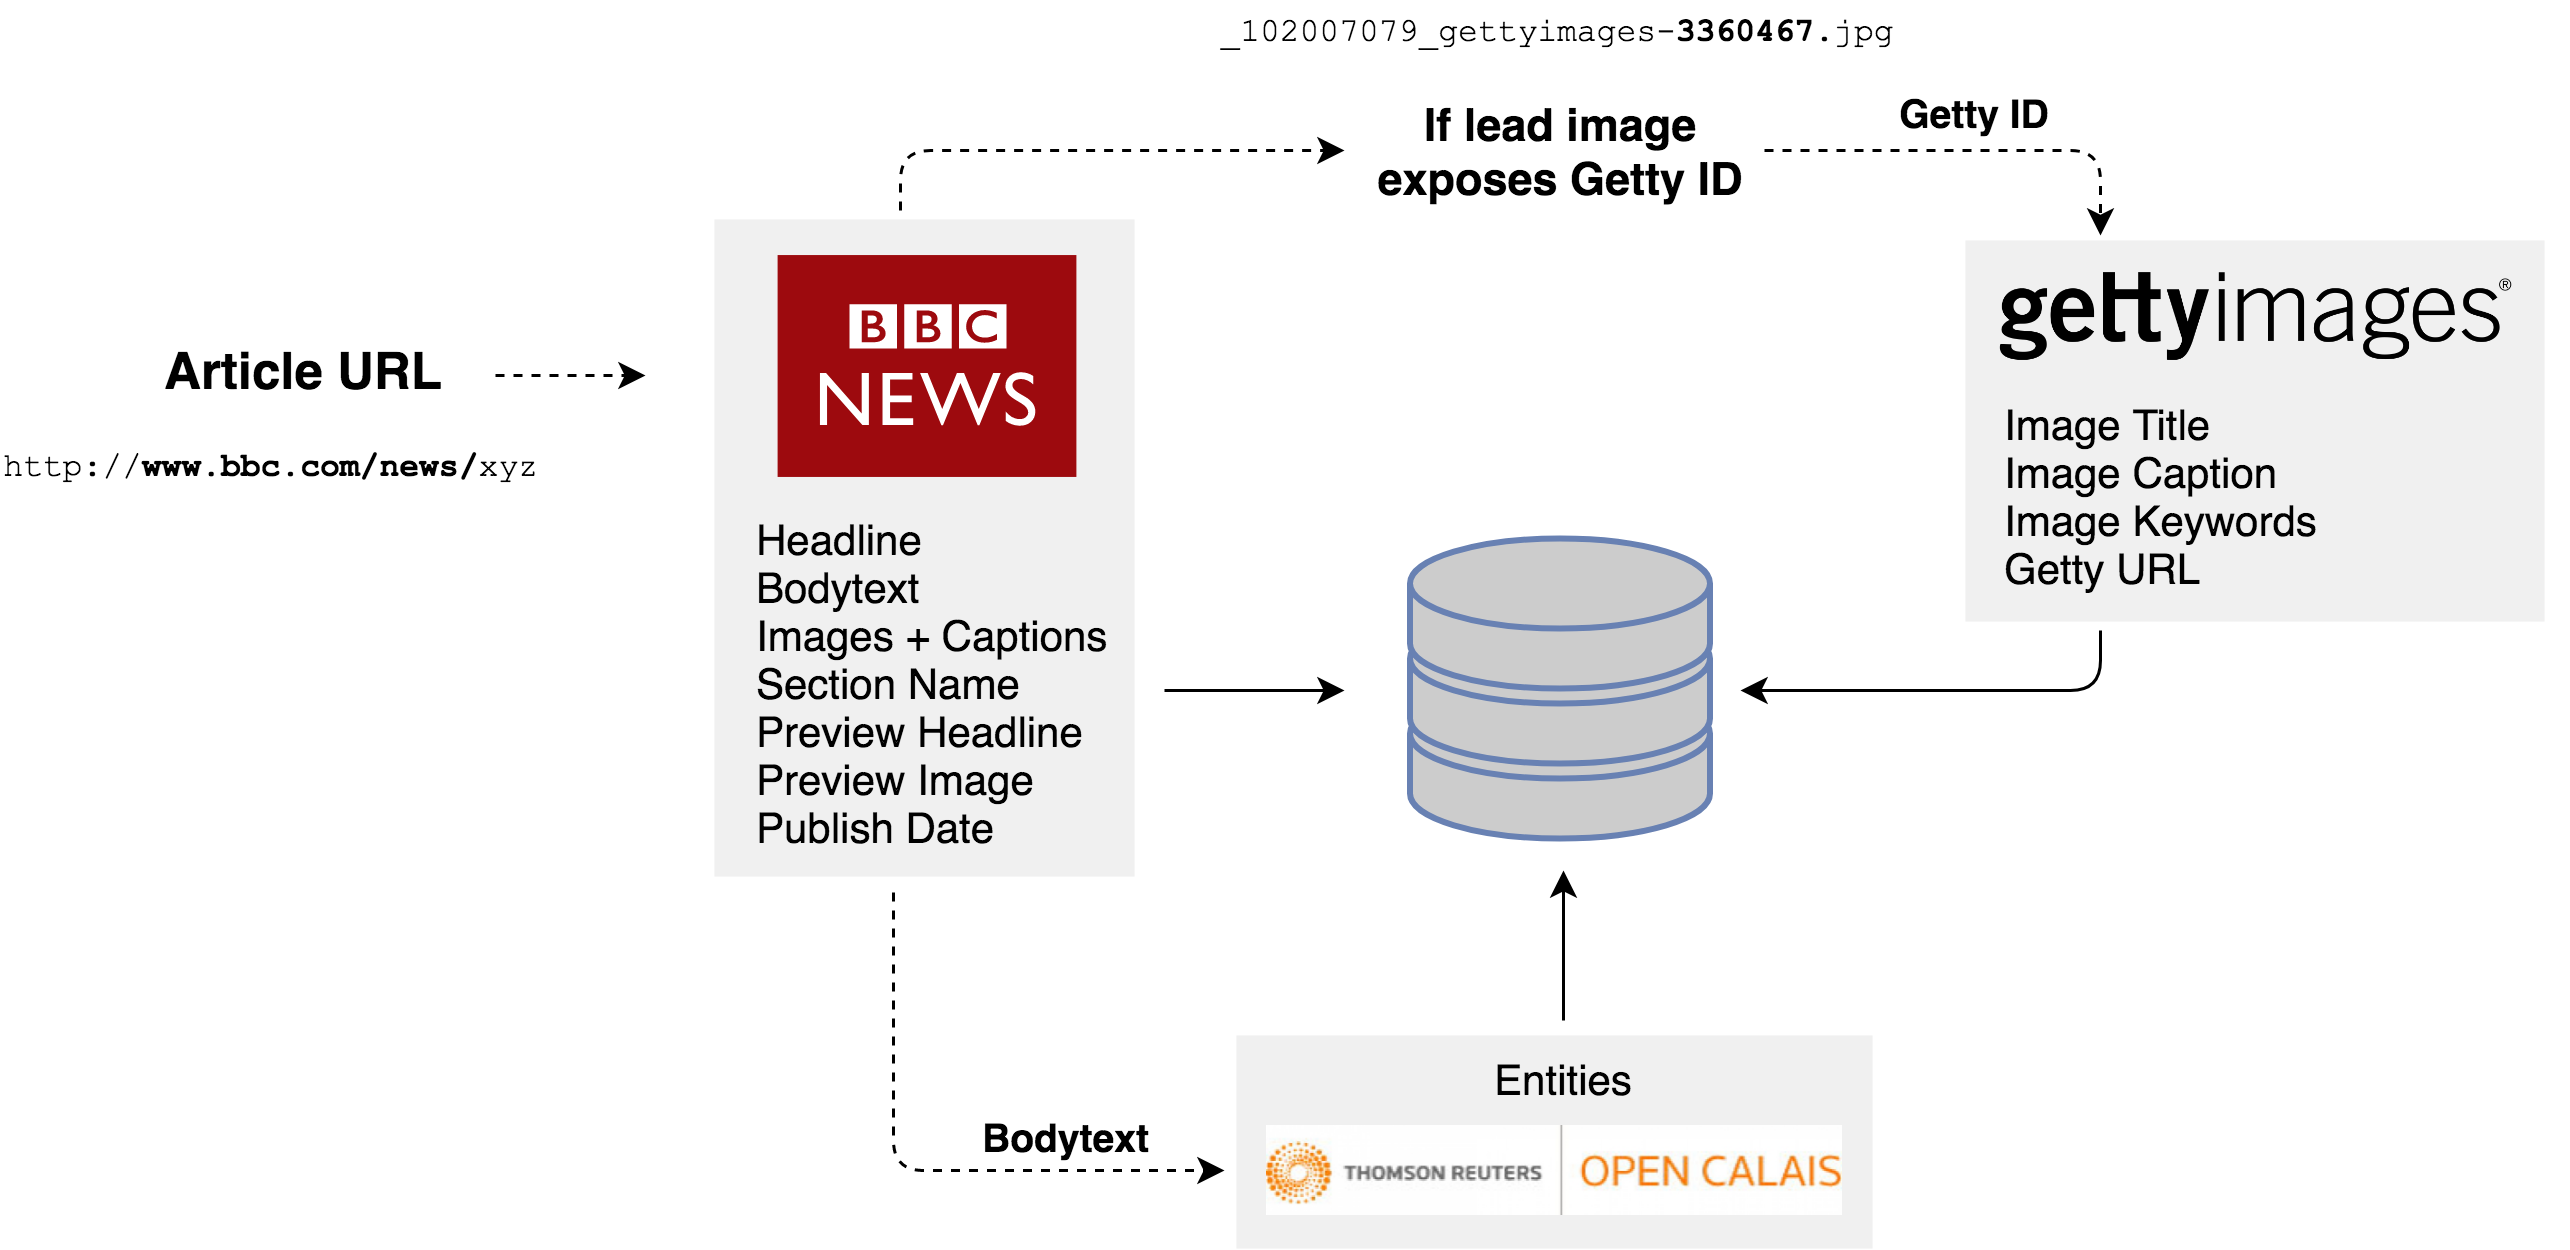
\includegraphics[width=\columnwidth]{picpic-scraper.png}
  \caption{Outline of the scraping procedure for one single article}
  \label{fig:picpic-scraper}
\end{figure}

The data set used for both training and evaluation of the system consists of two corpora. All images selected by the system are drawn from a large corpus published by the image agency \emph{Getty Images}. A collection of news articles was downloaded from the \emph{BBC News} website \cite{BBCBBCNews}.

Getty is particularly popular among media and news organisations worldwide and offers comprehensive coverage of contemporary news incidents, historical photography as well as stock photography. Using this corpus is therefore very close to a real-world application. Getty offers access to its image collection through an open web interface called "Getty Images API" \cite{GettyImagesAPIOverview} that is - with certain limitations - free to use. Besides this practical reason, Getty Images was chosen because it covers the whole range of possible images for news articles, from pictures of current events to symbolic pictures that illustrate abstract topics. From a developer's perspective, using the Getty API makes sense because it offers programmatic access to structured data ready to use and can be regarded as one instance of an arbitrary image database.

When news organisations publish an article, image meta data is usually not included. Knowing this meta data, however, is crucial for the proposed machine to learn from the selections human editors make, as will be seen in Section \ref{SystemTrain}. The challenge in collecting the article corpus was hence to find news articles that do not only contain an image by Getty but do additionally allow a conclusion about the original entry in Getty's database. It was found that many articles on the \emph{BBC News} website \cite{BBCBBCNews} do in fact expose the original IDs of the embedded Getty images via image file names in the HTML documents. For example, in the following file name

\begin{lstlisting}
_102007079_gettyimages-3360467.jpg
\end{lstlisting}

\noindent the Getty ID is \lstinline{3360467}. Likewise, BBC News is an applicable source with regards to contents: The website publishes a vast collection of typical news articles every day. It focuses on reporting current events in a short and informative way and aims at a broad audience without a special interest. It features reports from all over the world and from many different topics, thereby closely resembling the coverage Getty offers.

Based on these findings, a scraping application was designed that requests all articles from the BBC News website in a periodic fashion, stores them locally, checks for each article whether either the preview image or the first image in the article (i. e.  the lead image) exposes the original Getty ID, and if so requests the image meta data from the Getty API as well. The lead image restriction was imposed because on the BBC News website these are the images that come closest to what the proposed application is intended to select: One image that conveys the core message of the article.

The exemplified scraping work flow in Figure \ref{fig:picpic-scraper} shows that a third source was added: \emph{Thomson Reuters Open Calais} \cite{ThomsonReutersOpenCalais} is a web service that identifies persons, companies, events, products and many other entities in an unstructured text. By submitting the article text to Open Calais, some semantic information about the occurring entities could be stored alongside the plain article. More details on how Open Calais was used to improve the machine learning approach of this system will be presented in Sections \ref{SystemPreprocessCalais} and \ref{SystemClassificationML}.

The scraping application was deployed on 14 June 2018 and run each day on 9 a.m., 4 p.m. and 9 p.m. UTC. By 4 October 2018 it has collected 18,830 articles with their associated Open Calais entity tags. 1,578 of these articles contain a lead image that exposes the Getty ID, resulting in a set of training data consisting of approximately 500,000 terms and their associated features.

\subsection{Preprocessing an Article} \label{SystemPreprocess}

Processing an article written in natural language requires bringing structure to the unstructured text. Hence, this system contains a preprocessing component that turns the plain article text into a machine readable list of all the terms that occur in the text. Table \ref{table:term-examples} shows an example output of the preprocessor for a short piece of text. The exact steps the preprocessor performs are explained below.

\begin{table}[h!]
    \caption{Preprocessing result for "God helps those who help themselves."}
    \centering
    \begin{tabular}{|c|c|c|c|}
         \hline
         stemmed term & original terms & term frequency & first occurrence  \\
         \hline
         god          & God            & 1              & 0                 \\
         help         & helps, help    & 2              & 0.081             \\
         god help     & God helps      & 1              & 0                 \\
         help those who help & helps those who help & 1 & 0.081             \\
         \hline
    \end{tabular}
    \label{table:term-examples}
\end{table}

\paragraph{Tokenisation.} The first step is to turn the plain text, that is, a sequence of characters, into a sequence of words. This is achieved with a simple tokeniser that splits the original character sequence into substrings at every character that is neither an alphabetic letter, a digit nor an underscore. 

\paragraph{N-Gram Selection.} Since terms do not always consist of just one word, the preprocessor considers compounds consisting of up to four consecutive words as well, so called \emph{n-grams}. This is achieved by sliding a two, three and four word wide window over the previously generated list of words. However, only n-grams that do not overlap with a punctuation character (such as a full stop or a comma) are considered, i. e. n-grams must not exceed the borders of a clause. The n-grams are appended to the list of words.

\paragraph{Stopword Removal.} Many languages have words that convey little meaning on their own and can be left out from analysis, commonly referred to as "stopwords". In English these are mainly pronouns and particles such as "he", "themselves", "by", "when". The complete list of stopwords used in this system can be found in Appendix \ref{AppendixStopwords}. The preprocesor removes all these words from the word list, if they occur individually. Additionally, it removes any n-gram that starts or ends with a stopword, a procedure inspired by Hulth \cite{HulthImprovedKnowledge}.

\paragraph{Stemming.} In order to enable grouping of different inflections of the same word or closely related words, a procedure called "stemming" is applied to the complete word list. This refers to the reduction of words to their linguistic root. Porter's stemming algorithm \cite{Porter1980AnStripping} for the English language has proven to be reliable and effective and was hence chosen for this step.

\paragraph{Feature Assignment} After stemming, the preprocessor characterises each term with a set of features. The choice of features is a crucial part of the whole application, since these are the values the classifiers will use for deciding whether a term is a keyword or not. The features applied in this application are discussed in-depth in the following subsections.

\subsubsection{Features of a Term} \label{SystemPreprocessFeatures}

After the list of stemmed terms is assembled, many terms will occur more than once. Even though a simple measure, the frequency of a word does at least give some evidence about its importance for the text - an assumption fundamental to linguistic measures such as \emph{tf*idf} \cite{Salton1988Term-weightingRetrieval}. Manual benchmarks have largely confirmed this assumption for the BBC corpus on hand, which is why \textbf{term frequency} was included as the first, most basic feature for each term. The preprocessor eliminates duplicate words in the list by combining them to one list entry. It starts off by assigning a term frequency of 1 to each term and increments this count for each duplicate term it detects.

The most powerful term characteristic the manual benchmarks have revealed is the relative position at which a term occurs for the first time. The earlier a term is mentioned, the more important it seems to be for the story. This finding is not surprising, considering one of the basic writing techniques journalists use for presenting hard news: "placing the most important information at the beginning of the story, thus circumventing the reader's decision whether to continue or stop the reception." \cite[p. 501]{Pottker2003NewsAppear} This convention, commonly referred to as the "inverted pyramid" \cite[ibd.]{Pottker2003NewsAppear}, results in a decreasing amount of relevance over the course of a typical news article. Combined with term frequency, the \textbf{first occurrence} of a term rendered sufficiently good results for the statistical approach to be based on solely these two measures (see Section \ref{SystemClassificationStat}). In technical terms, this feature is implemented by searching the plain article text for the respective term and measuring the distance to the first character of the text relative to the total number of characters, i. e. a value of 0 refers to the first character in the article and 1 refers to the last.

Manual benchmarks were carried out for two other linguistic features, but the results were rather discouraging. A \textbf{part-of-speech} lookup in the WordNet database \cite{Fellbaum1998WordNet:Database} resulted in a 5-dimensional vector representing the number of nouns, verbs, adjectives, adverbs and other words in a term but did not reveal any pattern linked to image keywords in the benchmarks. It was therefore left out from this proposal. A feature called \textbf{paragraph type} was designed as a 4-dimensional vector that represents the number of times a term occurs in the headline, sub headlines, list items and regular paragraphs. Even though it seems likely that keywords occur in headlines and sub headlines, adding this feature actually blurred the results. BBC News uses sub headlines particularly often for inserting additional items into the article text that are not directly related, thus many words appeared to be keywords even though they were unrelated to the topic. All in all, the complications with this feature were outweighing the benefits, which is why it was chosen to drop it.

\subsubsection{Enhancing Preprocessing with Semantic Tagging} \label{SystemPreprocessCalais}

One of the key difficulties in preprocessing the articles for term classification was the correct aggregation of terms that refer to one and the same thing. Consider for example the fictitious person "Jane Smith" who acts as a lawyer in an article: This person could be referred to with a range of different terms such as "Jane Smith", "Ms Smith", "Jane", "the lawyer", "the attorney", "the procurator", "lawyer Jane Smith" or simply "she". Some of these terms could be captured with naive approaches such as reacting to the keywords "Ms", "Mrs" and "Mr" or integrating sub terms into enclosing terms (e. g. "Jane" into "Jane Smith"). But never would suchlike approaches encompass all possible mentions.

It was therefore decided to enhance the preprocessing component with the automated semantic tagging system \emph{Open Calais}. Open Calais is a "web service that attaches intelligent metadata-tags to [...] unstructured content" \cite[p. 1]{ThomsonReuters2018ThomsonGuide}. The service offered by the news agency \emph{Thomson Reuters} processes natural language with an engine based on statistics, machine learning and other heuristics, and is free to use. The tags it assigns include the overall topics of a text, entities occurring in the text and relations between these entities. Entities can be persons, companies, organisations, countries, events and many more. The proposed system only makes use of Open Calais' entity detection, ignoring topics and relations.

\begin{figure}[ht]
    \caption{Example for Open Calais entity detection \bigskip}
    \centering
    \begin{tabular}{l p{10cm}}
        Input text: & \nohyphens{\emph{"\underline{Marty Balin} - \underline{the co-founder} of the psychedelic rock band \underline{Jefferson Airplane} - has died aged 76, \underline{his} family and publicist say. They did not specify the cause of death of \underline{the US musician}."}} \bigskip \\
        
        Detections: & \begin{tabular}{|l|l|l|}
         \hline
         \textbf{entity name} & \textbf{exact terms}        & \textbf{entity type}       \\
         \hline
         United States      & US                            & Country           \\
         \hline
         Jefferson Airplane & Jefferson Airplane            & MusicGroup        \\
         \hline
         Marty Balin        & \pbox{50cm}{\vspace{.2\baselineskip}Marty Balin\\the co-founder\\his\\the US musician\vspace{.3\baselineskip}} & Person            \\
         \hline
         co-founder & co-founder & Position \\
         \hline
         US musician & US musician & Position \\
         \hline
    \end{tabular}
    \end{tabular}
    \label{table:calais-example}
\end{figure}

Adding this information to the system enables term aggregation way beyond the simple stemming explained above. As seen in Figure \ref{table:calais-example}, Open Calais detects even small references to entities that consist of just one pronoun. This has three major benefits: Firstly, it enables a more detailed elimination of duplicate terms in the list, since each term that is detected as belonging to an entity can be merged with all other terms belonging to the same entity. Secondly, by exposing an entity name, Open Calais offers a way of detecting which occurrence of the term actually describes the entity in the most common fashion (and is hence best for using in the image query). And lastly, it enables a more precise specification of term frequency, counting not only direct mentions of an entity, but also paraphrased references to it.

Thomson Reuters does not disclose the exact methods Open Calais uses, but it clearly states that machine learning is involved \cite{ThomsonReuters2018ThomsonGuide}. This is at odds with the definition of the statistical approach in the presented system (see Section \ref{SystemClassificationStat}), which is why the additional aggregation described above is only applied in the machine learning approaches.

\bigskip

Adding Open Calais entity detection to the system enables another modification for the machine learning approaches: Since Open Calais does not only detect entities, but also assign an entity type, another term feature can be introduced. Those terms that were detected to be entities get assigned the additional feature \textbf{entity category}. This feature is meant to describe what "kind" of term one is dealing with, with the assumption in mind that some types of entities are better search terms than others (e. g. a person might be preferred to a country or an organisation's name). In fact, research has shown that the great majority of image request newspaper journalists make are aimed at named persons, things and locations. \cite[p. 106]{Westman2006ImageContext} Open Calais knows 41 different entity types. In order to group together closely related entity types and to reduce complexity, they were combined into seven entity categories: Event, HumanProtagonist, OrganizationProtagonist, Position, Location, Product and Other. The exact grouping can be found in Appendix \ref{AppendixEntcats}. These group labels are then assigned as a feature value to each affected term.

\begin{table}[b]
    \caption{Entity categories for the terms in Table \ref{table:calais-example}}
    \centering
    \begin{tabular}{|c|c|c|}
        \hline
        \textbf{entity name} & \textbf{entity type} & \textbf{entity category} \\
        \hline
        United States & Country & Location \\
        Jefferson Airplane & MusicGroup & HumanProtagonist \\
        Marty Balin & Person & HumanProtagonist \\
        co-founder & Position & Position \\
        US musician & Position & Position \\
        \hline 
    \end{tabular}
    \label{table:entcat-example}
\end{table}

The actual benefit of adding these labels to the list of terms was not obvious in the manual benchmarks conducted before the implementation. However, their overall positive - yet not very strong - effect became visible in the evaluation of the implemented system that will be presented in Section \ref{Eval}. It remains to examine whether the information extracted by Open Calais can be used in a more advantageous manner than in this proposal. Some ideas towards deeper exploitation of semantic tagging can be found in Sections \ref{Limits} and \ref{Conclusion}.

\subsection{Training Neural Networks} \label{SystemTrain}

\begin{figure}[t]
  %% Datei auf ganze Breite des Texts vergrößert
  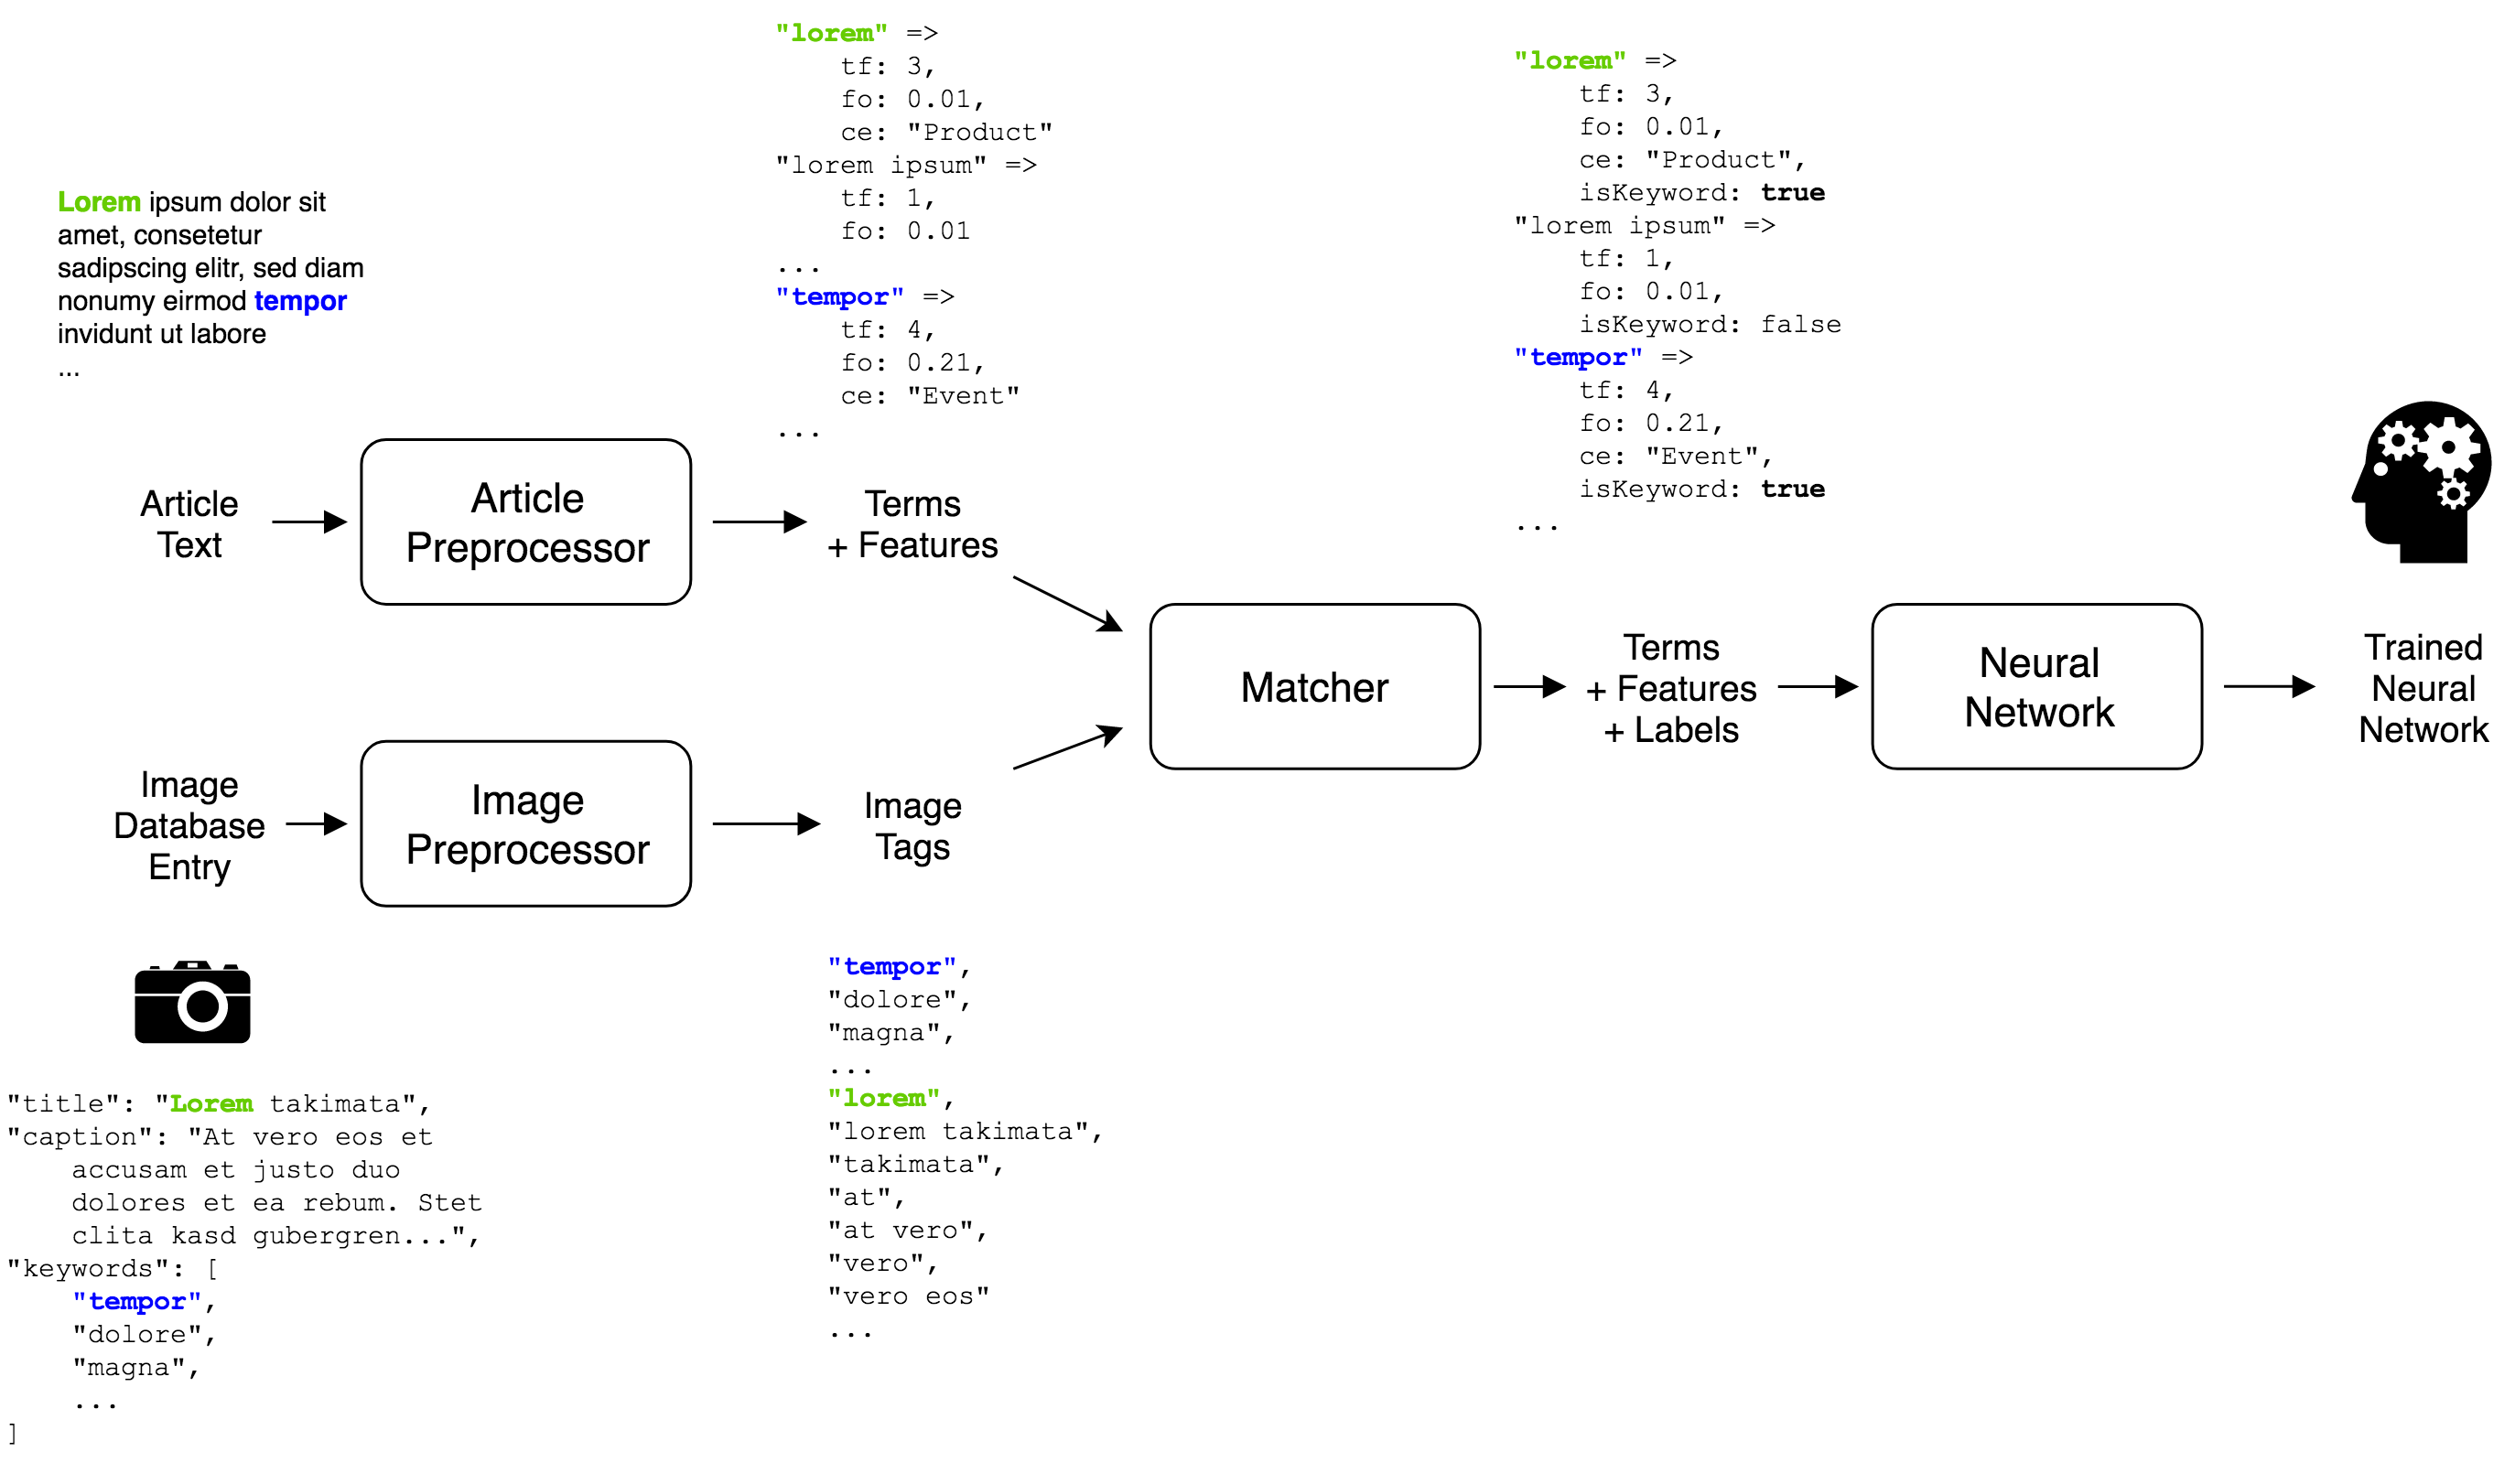
\includegraphics[width=\columnwidth]{picpic-training.png}
  \caption{Outline of the training pipeline}
  \label{fig:picpic-training}
\end{figure}

\begin{quote}
    "[L]earning is the process of converting experience into expertise or knowledge."
    
    \cite[p. 1]{Ben-David2014UnderstandingAlgorithms}
\end{quote}

\noindent Learning from real world observations is fundamental to one of the two approaches examined in this work, the machine learning approach. It is hence worth to discuss, which training data is necessary to gain the required knowledge, and how this data is generated in the proposed system. Referring to the quote by Ben-David above, the expertise this system is trying to gain is to distinguish between terms that are suitable for searching an image and terms that are not. So what would be the experience the system should make in order to develop this ability? Strictly speaking, it should learn from what human editors do when searching for an image. The ideal training data for the task at hand would thereby be a set of terms human editors have used for searching an image, united with another set of terms they did not use. It is immediately clear that such data is not readily available. Collecting it would take lots of time, since human editors would have to make thousands of image requests until enough data is available, not to speak of the privacy considerations such a surveillance would imply.

In order to avoid these difficulties and due to time limitations, this system is trying to substitute the missing data with a workaround. This workaround is based on the assumption that any combination of terms that occur in the description of an image would form a query good enough to return at least a similar image from the same database. This is, in a sense, a weak assumption, since there will always be terms in image descriptions that do not strictly set the image apart from unrelated images. But it helps getting as close as possible to actual search terms with the data available form the sources presented in Section \ref{SystemCorpus}.

In practice, the training data is generated from articles that have a Getty image as their lead image on the BBC website, or more precisely articles for which the scraper was able to download additional image meta data from the Getty API. Article text and image meta data are compared and all article terms that also occur in the image description are labelled as "keyword", whereas all other article terms are labelled as "no keyword". This procedure as well as the exact steps taken for training the networks are detailed in the following subsections. Figure \ref{fig:picpic-training} shows a schematic representation of the whole training pipeline.

\subsubsection{Preprocessing an Image for Training} \label{SystemTrainPreprocess}

\begin{figure}[t]
    \caption{Image meta data example}
    \centering
    \def\arraystretch{1.3}
    \begin{tabular}{l p{10cm}}
        \textbf{Image:} & \raisebox{-4.3em}[5.5em][5em]{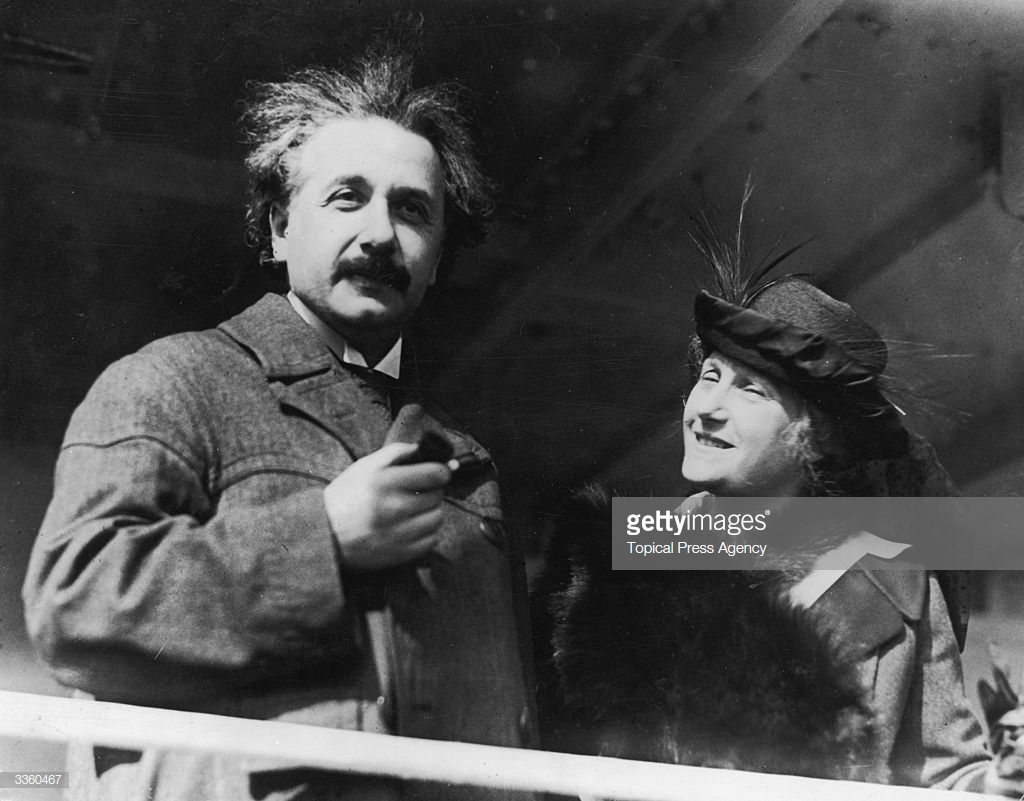
\includegraphics[width=.3\columnwidth]{einstein.jpg}} \\
        %\hline
        \textbf{Title:} & Einstein And Wife \\
        %\hline
        \textbf{Caption:} & circa 1921:  German-Swiss-American mathematical physicist Professor Albert Einstein (1879 - 1955) with his wife Elsa in Egypt.  (Photo by Topical Press Agency/Getty Images) \\
        %\hline
        \textbf{Keywords:} & \nohyphens{1990-1929, Adult, Africa, Black And White, Couple - Relationship, Data, Egypt, German Culture, Germany, Mathematical Symbol, Mathematics, People, Physicist, Science and Technology, Swiss Culture, Wife, Women, Albert Einstein, Elsa Einstein} \\
    \end{tabular}
    \label{fig:image-meta-example}
\end{figure}

\noindent To be able to match the article terms with the terms occurring in the image description, the image meta data has to be preprocessed with a procedure similar to the article preprocessor outlined in Section \ref{SystemPreprocess}. In doing so, a second list of terms is generated, so called image tags, that can then be compared to the article terms. The input data for this image preprocessor component consists of three fields - title, caption and keywords of the image - that have to be treated in two different ways.

\paragraph{Keywords} The Getty Images API provides a list of keywords that describes each image according to topics, content and some technical features such as orientation or colour (see Figure \ref{fig:image-meta-example} for an example). Since most of these keywords represent fixed terms, additional steps such as tokenisation and n-gram selection can be omitted. Except for stemming with Porter's algorithm, no preprocessing is applied to them.

\paragraph{Title and Caption} In addition to the structured list of keywords, the API provides a title (headline) and caption (description) for each image in natural language. In contrast to the keywords, title and caption explicitly describe the people and things depicted on an image. It can be assumed that terms occurring in title and caption are more likely to resemble queries human editors make, which is why it was decided to include them in the list of image tags. The preprocessing steps performed on these two fields are similar to the article preprocessor: Tokenisation, n-gram selection, stopword removal and stemming are applied in the same way as described in Section \ref{SystemPreprocess}, resulting in a list of caption terms.

Both lists are then merged so that the output contains no duplicate terms. The resulting list of image tags is passed on to a training data generator component described in the following section.

\subsubsection{Generating Training Data} \label{SystemTrainGenerate}

\begin{figure}[h]
    \caption{Example representation of one term as vector in the training data}
    \centering
    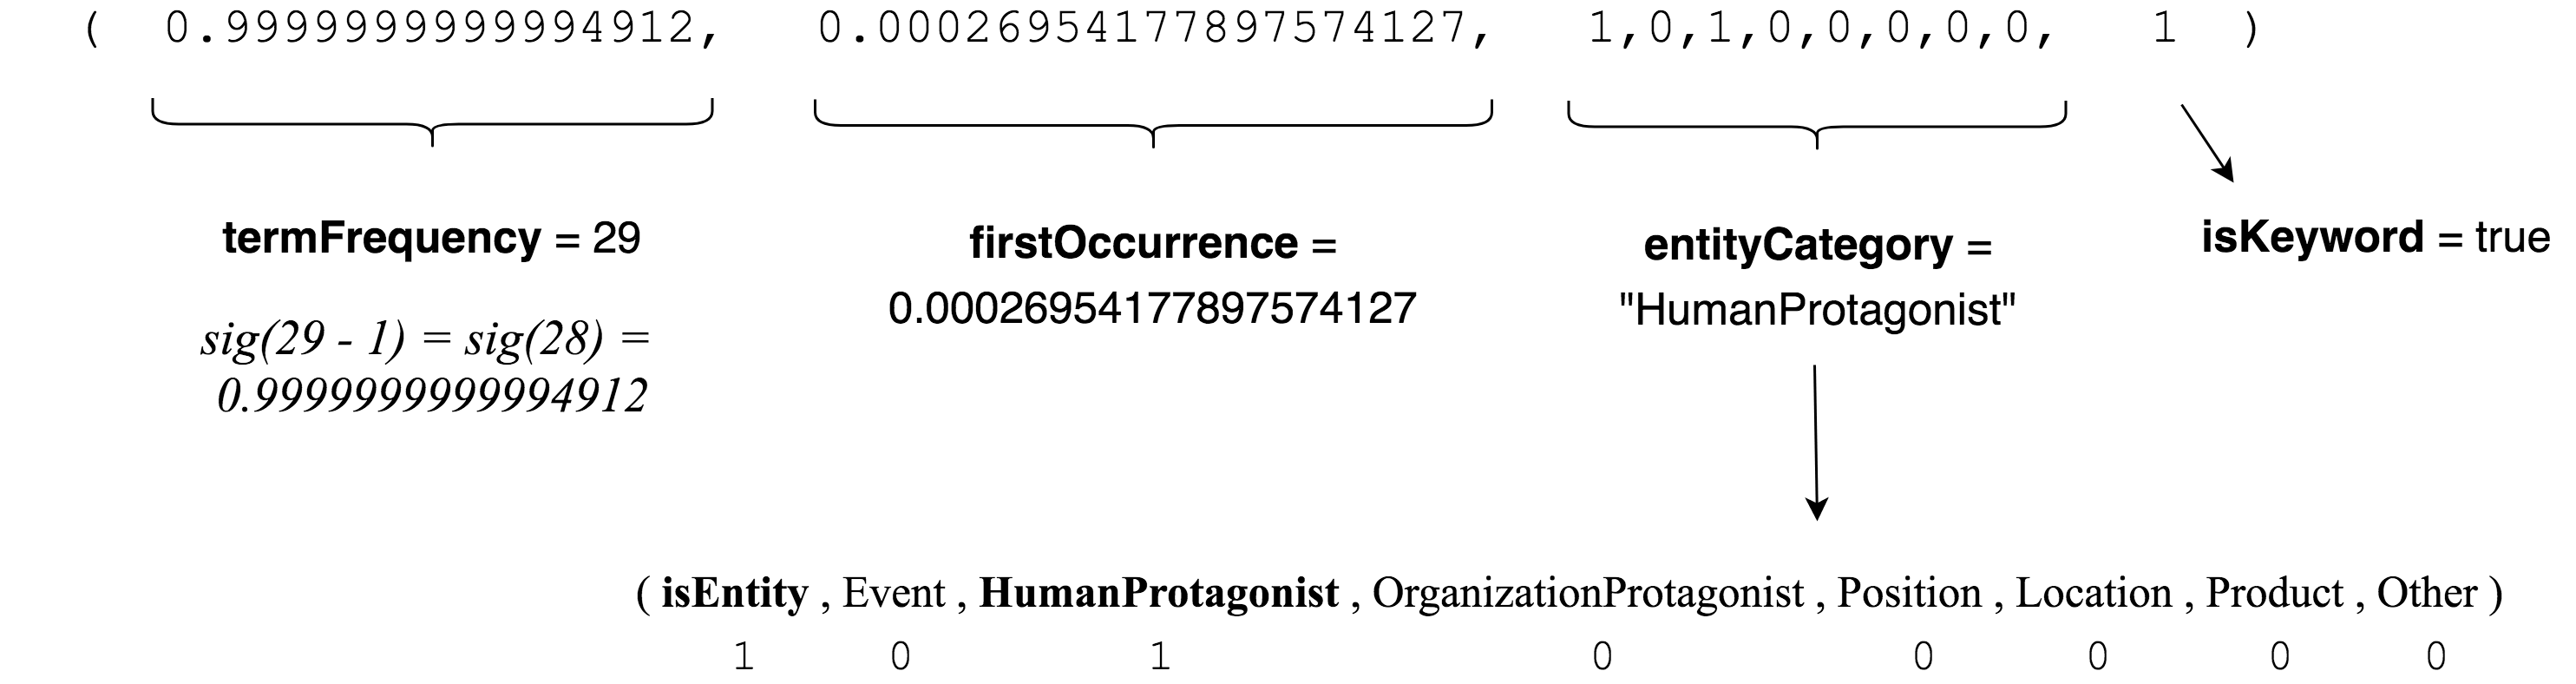
\includegraphics[width=\columnwidth]{example-training-term.png}
    \label{fig:example-training-term}
\end{figure}

\noindent At first, the training data generator component matches the list of article terms with the image tags. It assigns an additional boolean feature \textbf{isKeyword} to each term, with a value of \lstinline{true} for each article term that is also an image tag and \lstinline{false} for all other terms (see the "Matcher" component in Figure \ref{fig:picpic-training}). Subsequently, each term has to be transformed into a vector representing the input layer of a neural network. All feature values are mapped to numbers from the range between 0 and 1, with 0 representing an unactivated neuron and 1 representing a fully activated neuron. An example vector is shown in Figure \ref{fig:example-training-term}. The detailed transformations applied to each feature value are explained below.

\paragraph{Term frequency} This value is normalised with the sigmoid function:

\[
sig(x) = \frac{1 - e^{-x}}{1 + e^{-x}}
\]

\noindent Since the lowest possible value for term frequency is 1 (terms with a frequency of 0 would not occur at all), the value is decreased by 1 before applying the sigmoid function. This means that a term frequency of 1 will result in an unactivated neuron ($sig(1-1) = sig(0) = 0$). Sigmoid was chosen because its value increases quickly for natural numbers greater than 1. A term frequency of 4, for example, would result in an activation of $sig(4-1) = sig(3) \approx 0.9052$.

\paragraph{First occurrence} Values for this feature range from 0 to 1 by design and need no normalisation. They are adopted in the term vector unmodified.

\paragraph{Entity category} This feature can take seven different nominal values or no value at all. It is represented as an eight-dimensional vector on its own, where the first value expresses whether this term belongs to an entity or not (\emph{isEntity}) and the other seven values represent the entity categories (Event, HumanProtagonist, OrganizationProtagonist, ...). Figure \ref{fig:example-training-term} illustrates the pattern: If a term does not have an entity category assigned, all eight values are set to 0. If it has a category, \emph{isEntity} and the respective category dimension are set to 1. This representation was chosen because of the assumption that terms belonging to any type of entity might be better suited as search term than terms that do not belong to any entity. Whether this predication holds, is yet to be examined. 

\bigskip

\noindent Finally, one value representing the label is appended to the term vector: If the term was labelled as "keyword", this value is 1, otherwise it is 0.

\subsubsection{Training the Networks} \label{SystemTrainTrain}

\noindent All variations of the machine learning approach examined in this work use pre-trained feedforward neural networks for the classification of terms. Feedforward neural networks were chosen because they provide an easy mechanism to perform simple classifications, such as the task at hand. Since the search terms they predict can only be evaluated by humans looking at the selected images, there is no obvious benefit in remembering previous decisions, as for example recurrent neural networks do. All networks in this work consist of one input layer of varying size, one hidden layer sized proportionate to the input layer and one output layer consisting of two nodes, representing the two classes "keyword" and "no keyword".\footnote{For details on the structure of feedforward neural networks see \cite{Bishop1995NeuralRecognition}.} Varying the type and design of the networks is beyond the scope of this work and remains to be examined in future work. However, the software is designed to incorporate different types of networks in the future.

Four networks were trained for the evaluation in this work. Each of the examined networks uses a different combination of the term features to classify terms as "keyword" or "no keyword". These combinations are:

\vspace{-.5em}
\begin{itemize}
    \setlength\itemsep{0em}
    \item term frequency + first occurrence
    \item term frequency + entity category
    \item first occurrence + entity category
    \item term frequency + first occurrence + entity category
\end{itemize}
\vspace{-.5em}

\noindent Note that the combination of features determines the size of the input layer: Depending on which features are included, the term vector (see Section \ref{SystemTrainGenerate}) differs in length, and so does the number of nodes in the input layer.

For each feature combination, a separate set of 100,000 training terms from the BBC News corpus was generated with the procedure explained above. The implementation uses a third-party library (see \cite{BrainJSBrain.js:JavaScript}) for training the networks with the generated data.

\subsection{Term Classification} \label{SystemClassification}

Having preprocessed the article and trained the neural networks, the system is ready for performing the central step of the whole image selection process: All terms the article preprocessor has identified as keyword candidates are are now classified regarding their suitability as keywords. Instead of assigning an actual class to them, a probability value is calculated for each term. This value expresses the likeliness of the term being an appropriate search term. A probability value of 1 means that the system is 100 percent confident that the considered term is a search term. 0, in turn, means the system is entirely sure that the term is not a search term. Usually, this value does not reach its extrema.

The method used for predicting the probability values is interchangeable. This system compares five different methods: Four variations of neural networks as described in the previous section (referred to as the machine learning approach) and one method based on a simple calculation (the statistical approach). Whilst the neural networks do not reveal the patterns they follow by design, the statistical approach is designed with certain assumptions in mind, all of which are detailed in Section \ref{SystemClassificationStat} below. 

At the end of the classification step, a sorted list of terms descending by their probability values is forwarded to the query generator component.

\subsubsection{Statistics Based Approach} \label{SystemClassificationStat}

After discarding part-of-speech and paragraph type as features, only two features remain for calculating probabilities with statistical measures. The calculation applied is based on two assumptions:

\begin{enumerate}
    \item The more often a term occurs in an article, the more distinctively it describes its content.
    \item The earlier a term occurs for the first time, the more central it is for the article.
\end{enumerate}

\noindent Combining both assumptions, the ideal keyword in this model would be a term that occurs right at the beginning of an article and that is the most frequent term in the article. This is expressed in the following formula:

\[
p(tf, fo) = \frac{tf}{max(TF)} * (1 - fo)
\]

\noindent where $tf$ denotes the frequency of a term, $fo$ its first occurrence value, $max(TF)$ the highest term frequency value of all terms in an article and $p$ the probability of this specific term being a keyword. The fraction $\frac{tf}{max(TF)}$ equals 1 when the term under consideration is the most frequent one of the article, in all other cases it is less than 1. The difference $(1 - fo)$ converges towards 1 if $fo$ converges towards 0, i. e. the earlier a term occurs, the closer to 1 this part of the formula gets. The ideal keyword in this model would therefore have a probability value of $\frac{max(TF)}{max(TF)} * (1 - 0) = 1 * 1 = 1$.

What makes this approach stand out from the other approaches is its computational simplicity. The computing time for this basic formula is negligible, making this method exceedingly efficient. On the other hand, this approach involves no kind of semantic understanding of the text. Relying solely on two statistical measures and two strong assumptions makes it prone to miscalculations of seemingly important but redundant terms. Surprisingly, this approach has selected similar terms as the neural networks in many cases. Nevertheless, it was outperformed by some of the networks, as can be seen in the evaluation results in Section \ref{EvalResults}.

\subsubsection{Machine Learning Based Approach} \label{SystemClassificationML}

As most of the details regarding the design of the machine learning approach have been laid out in the previous sections, this section will briefly sum up the key differences to the statistical approach. By design, the machine learning approach is open to find its own patterns in the training data. In contrast to the statistical approach, no preassumptions were made about the features and their connections to keyword probabilities. Furthermore, the machine learning approach follows a more sophisticated preprocessing procedure than the statistical approach that solely relies on simple n-gram selection and stemming. By adding semantic understanding to the preprocessor, real-world entities are grouped to one single term, making these entities stand out more from less meaningful terms. Lastly, an additional feature called "entity category" is introduced in the machine learning approach, representing a rough categorisation of terms in events, different types of protagonists, professional positions, locations, products and other terms.

\subsection{Image Query} \label{SystemQuery}

The last processing step is to turn the ranked list of terms into a query string. Simply choosing the highest ranked term proved to be prone to errors, therefore several additional steps are proposed for this procedure. The observations made when selecting only one term correspond to the findings of Aramini et al.:

\begin{quote}
"We noted that using a single keyword would result in a too generic query, as it can represent a too generic concept. Furthermore, if we use a combination of two words, rather than only one, we drastically reduce the problem of polysemy. In fact the second word specifies the meaning of the first one, defining the context of the query." \cite[p. 142]{Aramini2015AutomaticImages}
\end{quote}

For this reason, the proposed system selects the two highest ranked terms by default and concatenates them to a query. However, it was found that queries of more than three words are too specific for the Getty API, resulting in many empty responses. Thus, if the resulting query consists of more than three words, the shorter term is dropped, even if it was ranked higher than the longer term, preserving the highest specificity possible.

Moreover, it was noted that due to the strong distinctive power of the term frequency feature, abbreviations and short forms were in many cases ranked higher than the spelled out terms - which would in turn be more suitable for the query. However, the spelled out terms usually follow shortly after the short forms in the ranking, since they tend to occur earlier. Hence, a simple heuristic is introduced that is meant to replace short forms with the spelled out terms, if they are ranked reasonably high.

\begin{figure}[h]
    \caption{Example for term replacement during the query generation}
    \centering
    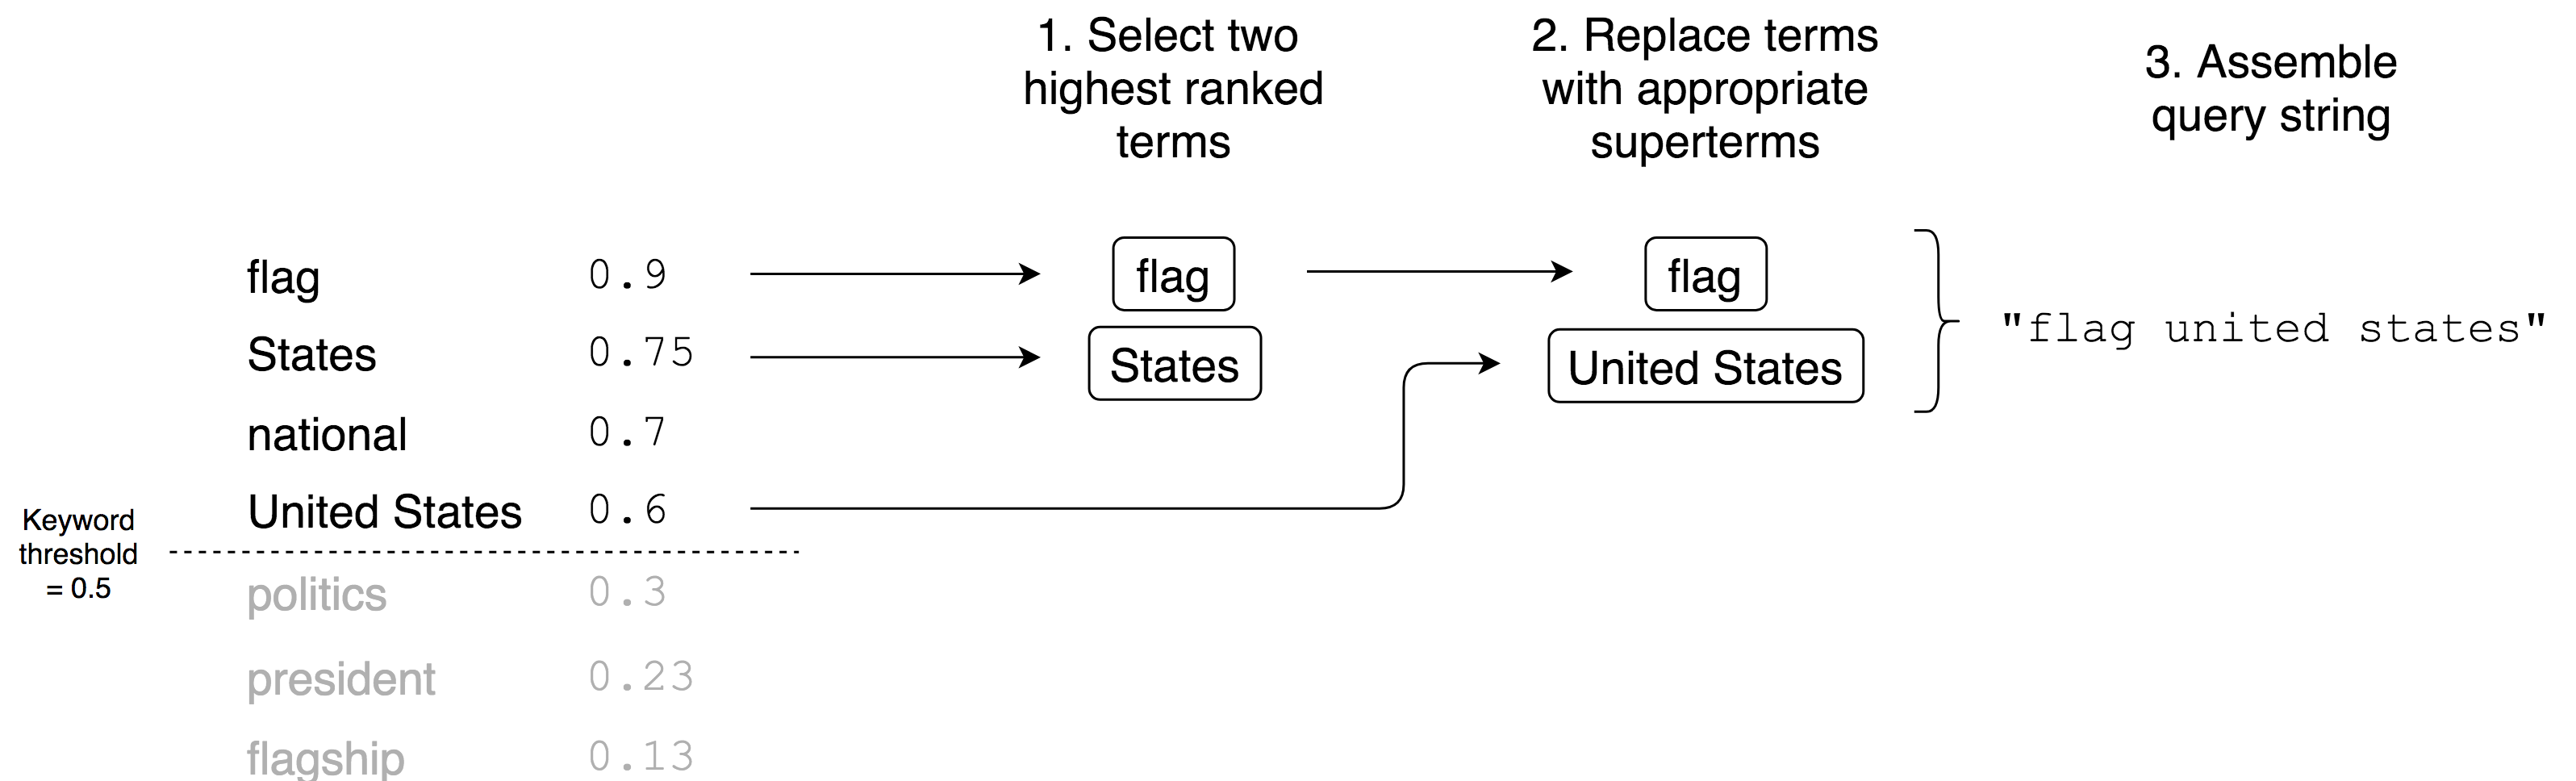
\includegraphics[width=\columnwidth]{picpic-querygen.png}
    \label{fig:example-querygen}
\end{figure}

Figure \ref{fig:example-querygen} shows this procedure in an exemplified manner: Firstly, a threshold probability value is defined. All terms with probabilities above this threshold are considered appropriate search terms, all others are discarded. After conducting manual benchmarks, the threshold was set to 0.5 for the statistical approach and 0.1 for the machine learning approaches. Then the two highest ranked terms are selected. For each of the selected terms, the query generator checks if there is another appropriate term that fully contains the selected term (called superterm below). In the example, "States" is replaced with its superterm "United States". "flag", in turn, is not replaced, even though "flagship" is a superterm. "flagship" has a probability of 0.13, which is below the defined threshold of 0.5. Finally, the query is generated by concatenating the resulting terms and converting them to lowercase letters. Note that in this example the search term consists of exactly three words. If it were four or more words, the shorter of both terms would be left out from the query. If both terms were of the same length, the second one would be discarded.

Finally, the query is sent to the Getty API, which returns a list of images sorted by their popularity. The most popular image is selected as an illustration for the article. Other options would be to sort the images by date or by "best match", neither of which did appear to render similarly good results in manual tests.

\

%______________________________________________________________________

\cleardoublepage

\section{Evaluation} \label{Eval}

Measuring the performance of a system that automatically selects images for news articles is not trivial. This task raises questions such as: What defines an appropriate image for an article? Is it only appropriate to show things that are mentioned directly in the text? Can an image be inappropriate even though it shows some entity from the text? Can it also be a good choice to select pictures that go beyond the text? What is more, who should judge on the quality of an image selection? Are news readers the best evaluators because they are the ones the news are made for? Or journalists because they have professional criteria and they are used to the selection task? Neither of both?

The evaluation of the system presented here takes a rather cautious approach. Since five different classification methods had to be evaluated, with potentially more to come in the future, the goal was to create a measure as objective as possible that is still applicable with reasonable effort. The experiment conducted for this work focuses merely on the factual correctness of image selections, leaving aside judgements on the journalistic quality of an image as well as considerations about how images could be perceived.

The following subsections give an overview of the evaluation method applied here. Section \ref{EvalFacts} explains the model for factual correctness that was employed in the experiment. Section \ref{EvalDesign} outlines how the experiment was conducted. Finally, experimental results are presented in Section \ref{EvalResults}.

\subsection{Factual Correctness as a Measure for System Performance} \label{EvalFacts}

Research has found that journalists use a variety of criteria for judging on the quality of an image. While it is most important that the image depicts the \emph{right} thing, they also pay heed to, for example, whether the image fits the allocated space (especially on newspaper pages, but also on websites), has certain visual features (good lighting, aesthetic composition), goes well with the article's headline, conveys the right mood and has eye-catching qualities. \cite[p. 108]{Westman2006ImageContext} Some of these criteria can not be applied in the evaluation of a general purpose system like the one at hand. Some others can only be assessed by professional photographers or journalists.

Due to time constraints and for reasons of efficiency, it was decided to focus on the most basic, yet most important criterion employed in practice: \emph{what} the image shows (see Westman et al.'s study on journalist's image search behaviour, \cite{Westman2006ImageContext}). In particular, this evaluation verifies that the content of the selected images is factually correct with regard to the article they are meant to illustrate. This can be seen as the minimum requirement for the system at hand: If the image is not factually correct in the majority of cases, the system can not be regarded as ready for production.

An image in this context is regarded as factually correct in relation to a news article, if one of the following criteria is matched:

\begin{enumerate}
    \item The image shows a real-world entity that is mentioned directly in the core message of the article.
    \item The image shows a real-world entity that is closely related to, or symbolises one the entities and concepts that form the core message of the article.
\end{enumerate}

An \emph{entity} in this definition can be something of physical existence (such as a person, a building, a plane) or an event (such as a demonstration, an inauguration, a press conference).

A \emph{concept} is something without physical existence that is nevertheless commonly regarded as one discrete instance, such a stock price, a presidency or the termination of a contract.

The \emph{core message} of an article is the piece of newsworthy information that sums up the article in one sentence. In journalism practice, this is sometimes referred to as the "lede" or the "nut graph" of a story. (see e. g. \cite[p. 110]{Rich2015WritingMethod})

As an addition to the above definition, an image is also regarded as factually wrong if it is not a photograph (but e. g. a drawing or a graphic).

\subsection{Evaluation Design} \label{EvalDesign}

Experiment and evaluation were carried out manually by the researcher. From the BBC corpus, a sample of 100 articles that match the following three criteria was selected:

\begin{enumerate}
    \item The original article is illustrated with a lead image by Getty. This restriction was imposed to make sure that Getty actually has a fitting image for all examined articles in its database.
    \item The article is written in news style. This condition applies to almost every article on BBC News. But since some of the assumptions underlying the system are made based on traditional news writing style, all other types of articles (such as features or listings) had to be sorted out for evaluation. This affected six articles in total.
    \item The article is among the 100 most recent articles to which the above conditions apply. If time is not specified, Getty's search API tends to return images from recent events first. In order to reduce the potential bias caused by this mechanism, only recently published articles were examined.
\end{enumerate}

\noindent For each selected article, a core message was formulated according to the definition given in Section \ref{EvalFacts}. These core messages answer the central questions for a news article: who, what, when, where, why and how? All examined articles with their respective core messages can be found on the CD attached to the printed version of this work.

The independent variable in this experiment is the approach used for classifying the terms. The following five approaches were examined:

\begin{itemize}
    \setlength\itemsep{0em}
    \item Statistical approach (abbreviated \emph{stat})
    \item Machine learning approach using term frequency and first occurrence (\emph{tf+fo})
    \item Machine learning approach using term frequency and entity category (\emph{tf+calais})
    \item Machine learning approach using first occurrence and entity category (\emph{fo+calais})
    \item Machine learning approach using term frequency, first occurrence and entity category (\emph{tf+fo+calais})
\end{itemize}

\noindent The dependent variable is the factual correctness of the image selection the system makes when one of the above approaches is applied. All other parameters in the system were kept constant throughout the entire experiment.

For each of the 100 articles, the image selection was run with all five approaches. Each resulting image was classified manually as either "factually correct" or "factually incorrect" according to the definition given in Section \ref{EvalFacts}. If the system returned no image, a "no image" label was assigned to the respective run. A comprehensive list of examined articles, core messages, selected images and classifications can be found on the attached CD.

\subsection{Evaluation Results} \label{EvalResults}

\begin{figure}[t]
    \caption{Image selection results for all approaches}
    \centering
    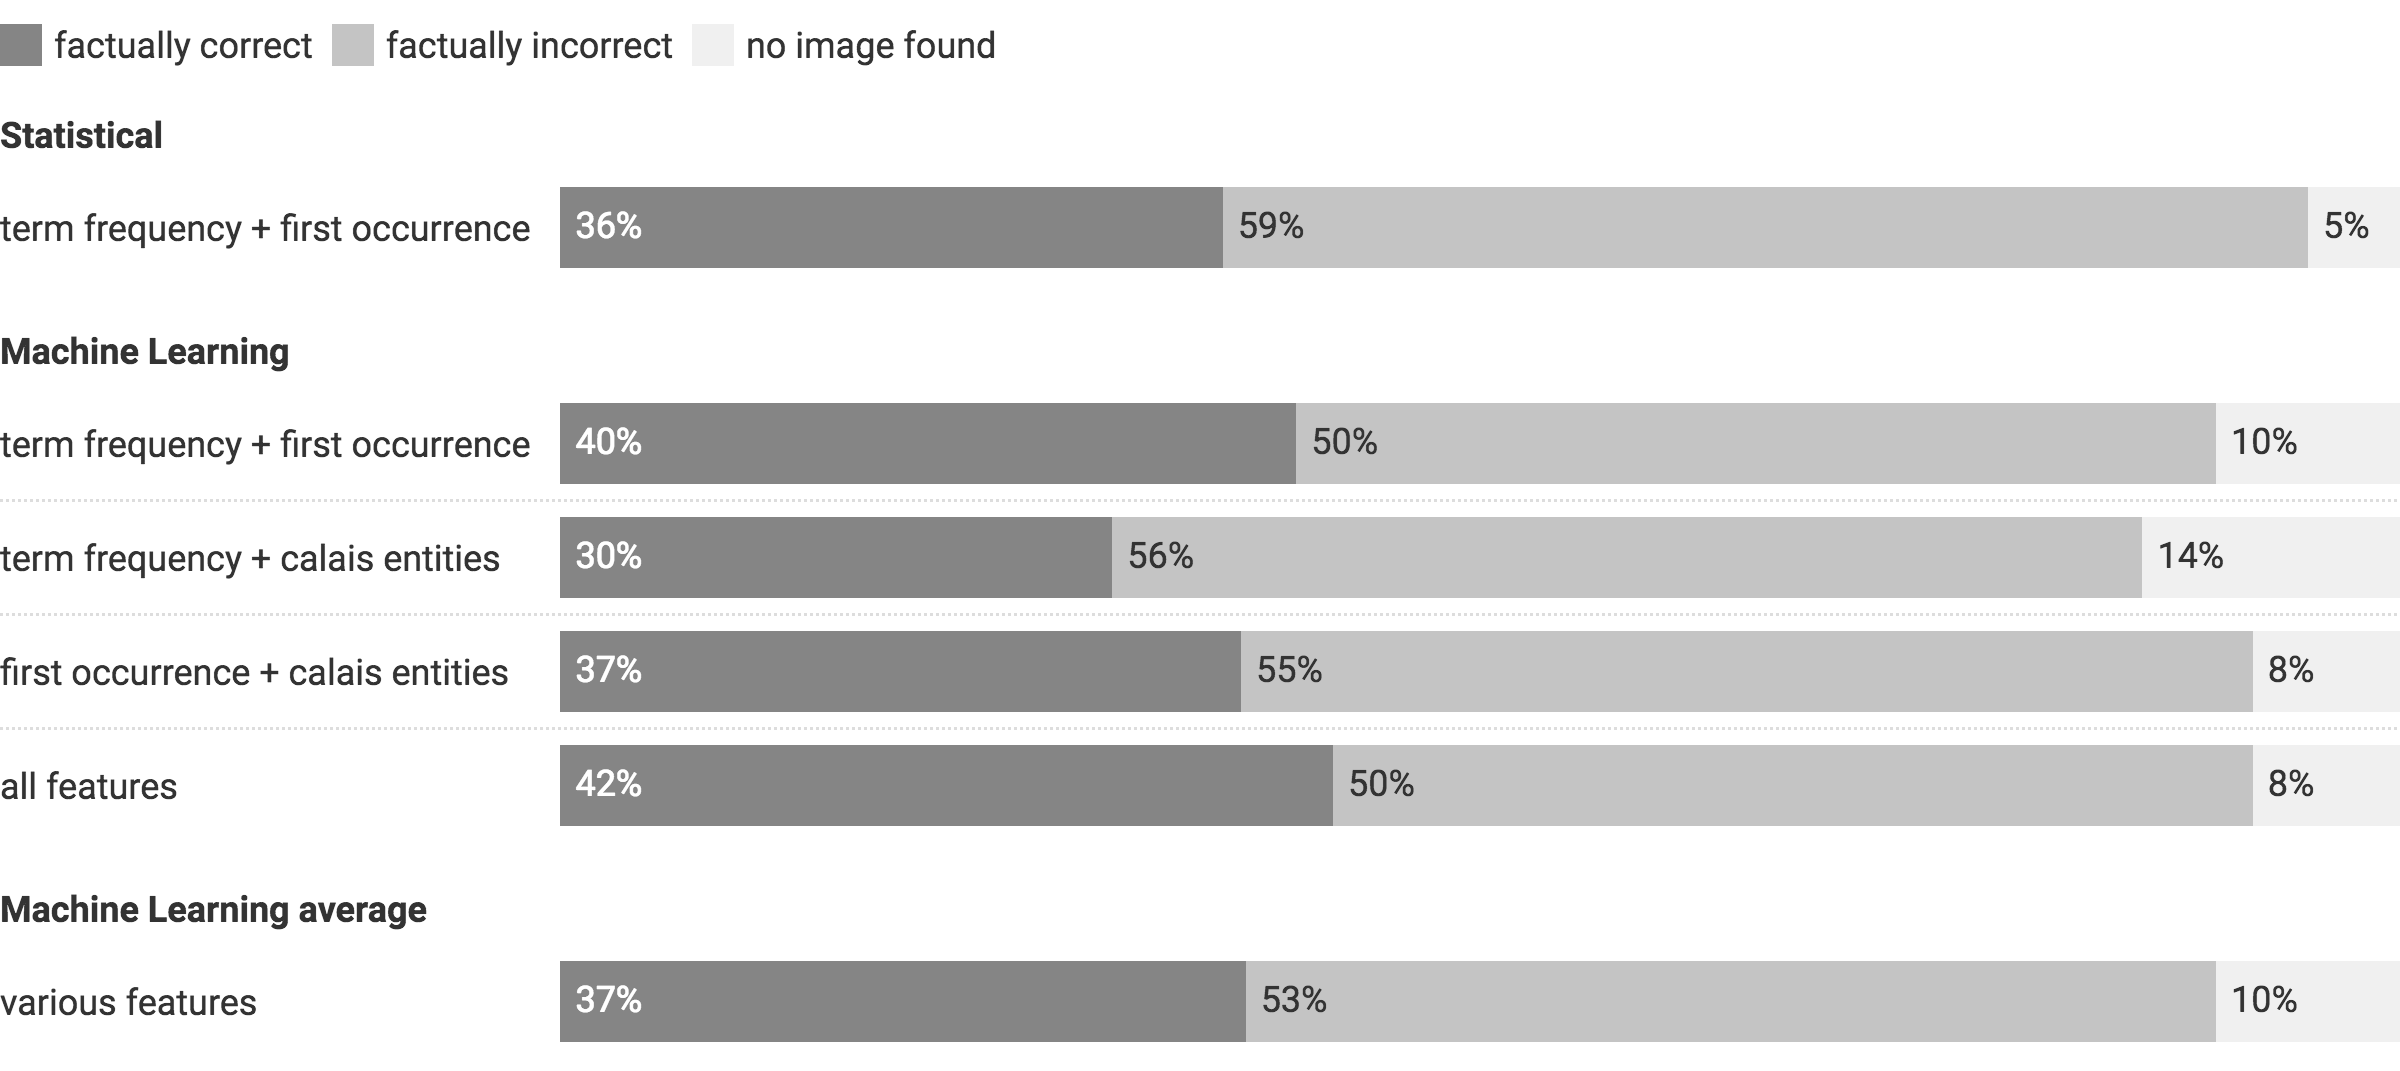
\includegraphics[width=\columnwidth]{fig-results-overview.png}
    \label{fig:results-overview}
\end{figure}

The main finding arising from the evaluation results is that the system can not be regarded as ready for production in its current state. On average, only 37 \% of all articles got a factually correct image assigned, 54 \% had a wrong image assigned and for 9 \% of the articles the system did not find an image at all.

Figure \ref{fig:results-overview} shows that the machine learning approaches performed similarly well as the statistical approach on average. However, results of the machine learning approach are significantly better when term frequency and first occurrence are both used as features: \emph{tf+fo} returned 40 \% correct images and \emph{tf+fo+calais} returned 42 \% correct images, which makes it the best performing approach in the experiment. At the other end of the spectrum ranks another machine learning approach: \emph{tf+calais} showed by far the worst performance in the experiment, selecting correct images for less than a third of all articles, having the highest rate of wrong articles of all machine learning approaches and returning no image for 14 \%. This highlights the importance of the first occurrence feature that will be examined in more detail below.

Even though similar to the average machine learning approach, in direct comparison \emph{stat} ranks at the lower end of the spectrum as well, as shown in Figure \ref{fig:stat-comparison}. It has the second lowest quota of factually correct images, with only \emph{tf+calais} performing worse. Furthermore, with 59 \% it has the highest rate of wrong images. This might also be due to its high efficiency: Whereas the machine learning approaches tend to return no image more often, \emph{stat} only returned no image in 5 \% of cases. It can be assumed that it is better to return no image instead of a wrong image in news publishing, where factual correctness has a high priority. So the seemingly good result that \emph{stat} is the most effective approach must actually be interpreted as possibly problematic.

\begin{figure}[h]
    \caption{Performance of statistical approach compared to machine learning approaches}
    \centering
    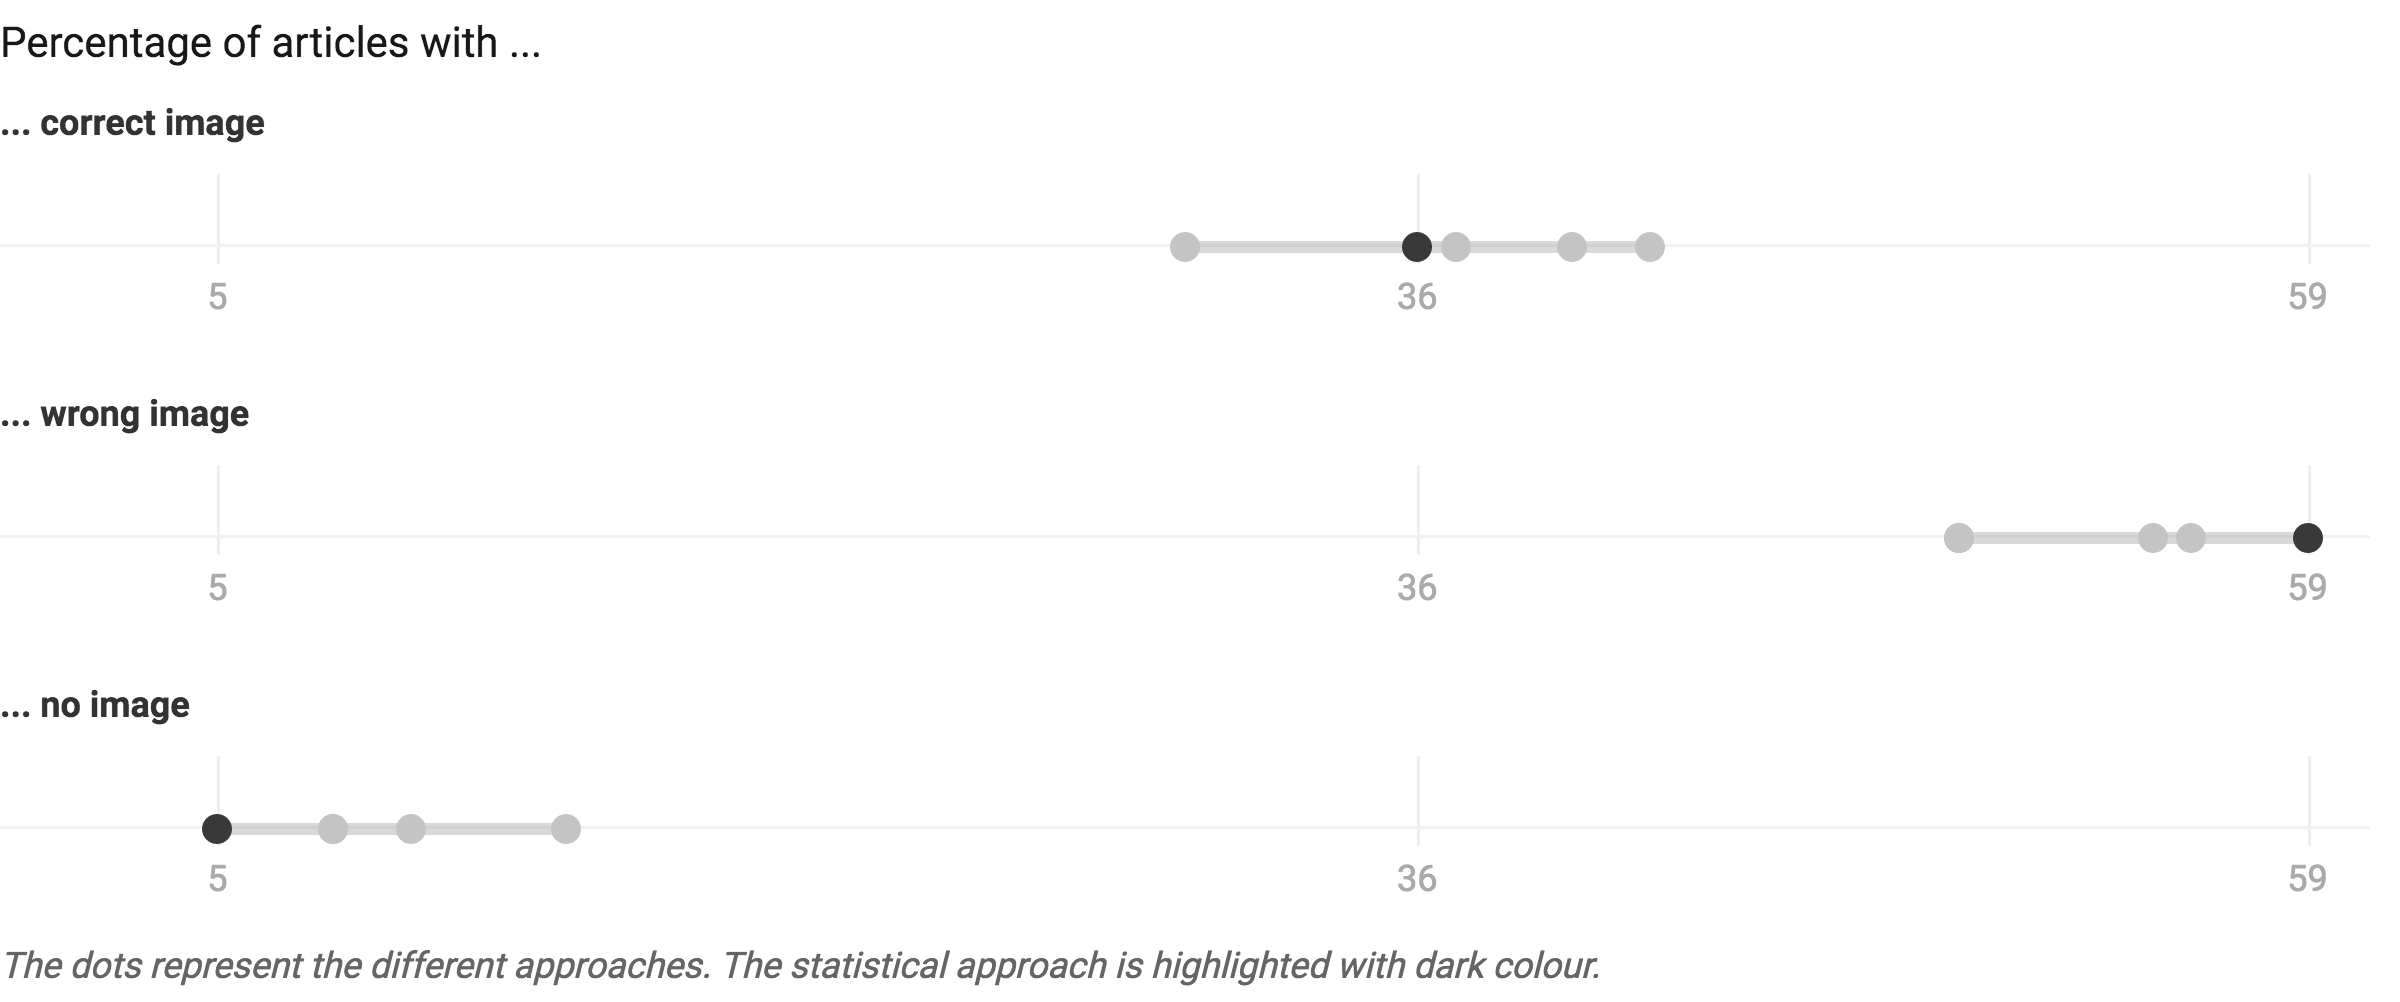
\includegraphics[width=\columnwidth]{fig-stat-comparison.png}
    \label{fig:stat-comparison}
\end{figure}

\begin{figure}[h]
    \caption{Influence of features on neural network performance}
    \centering
    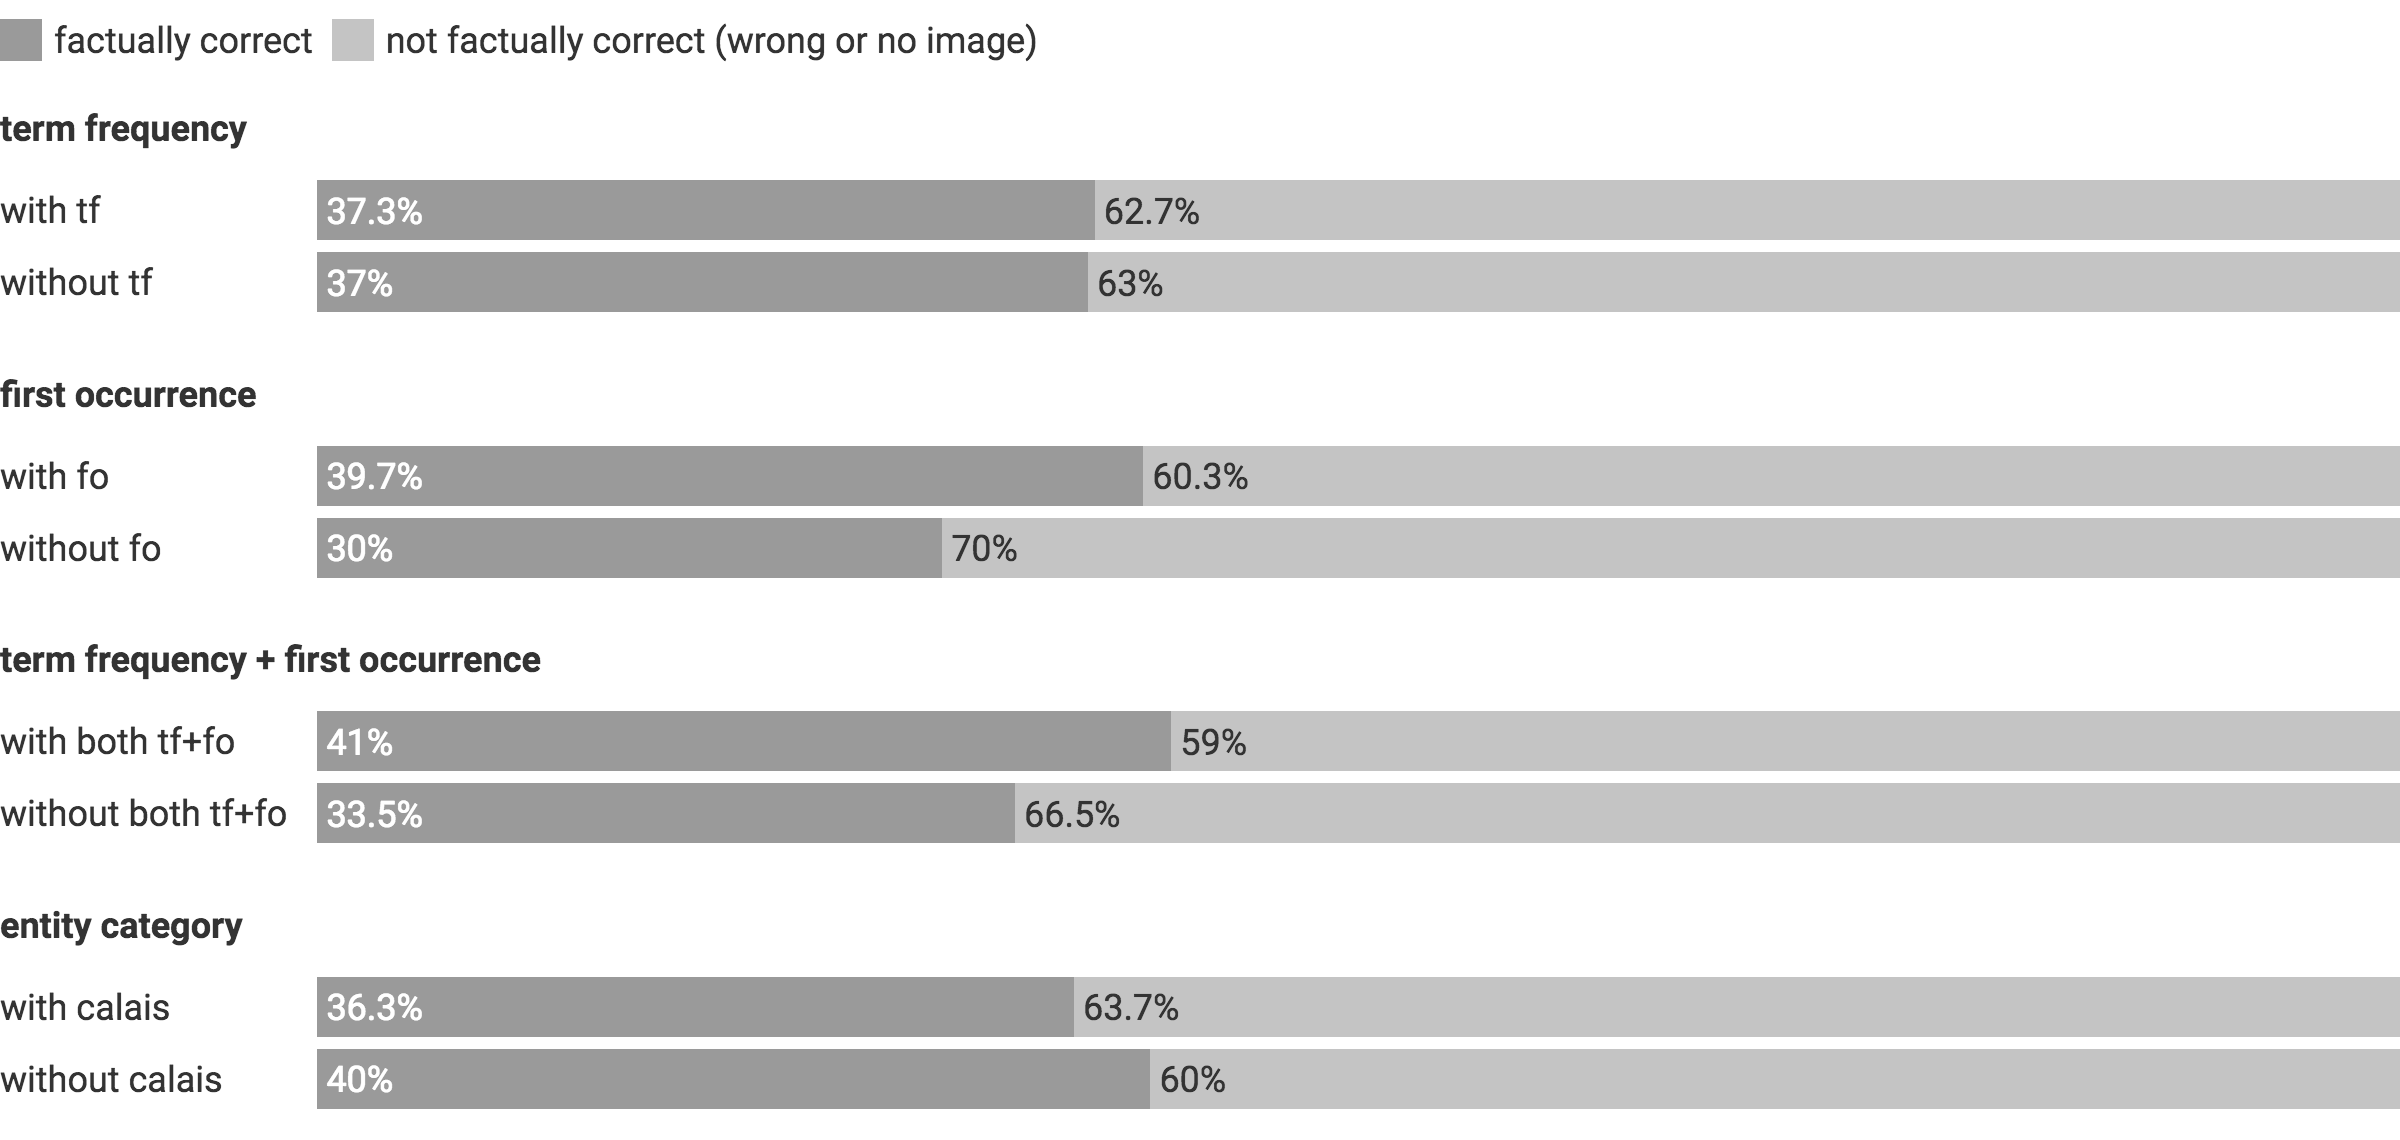
\includegraphics[width=\columnwidth]{fig-feature-influence.png}
    \label{fig:feature-influence}
\end{figure}

\begin{figure}[h]
    \caption{System performance per article topic}
    \centering
    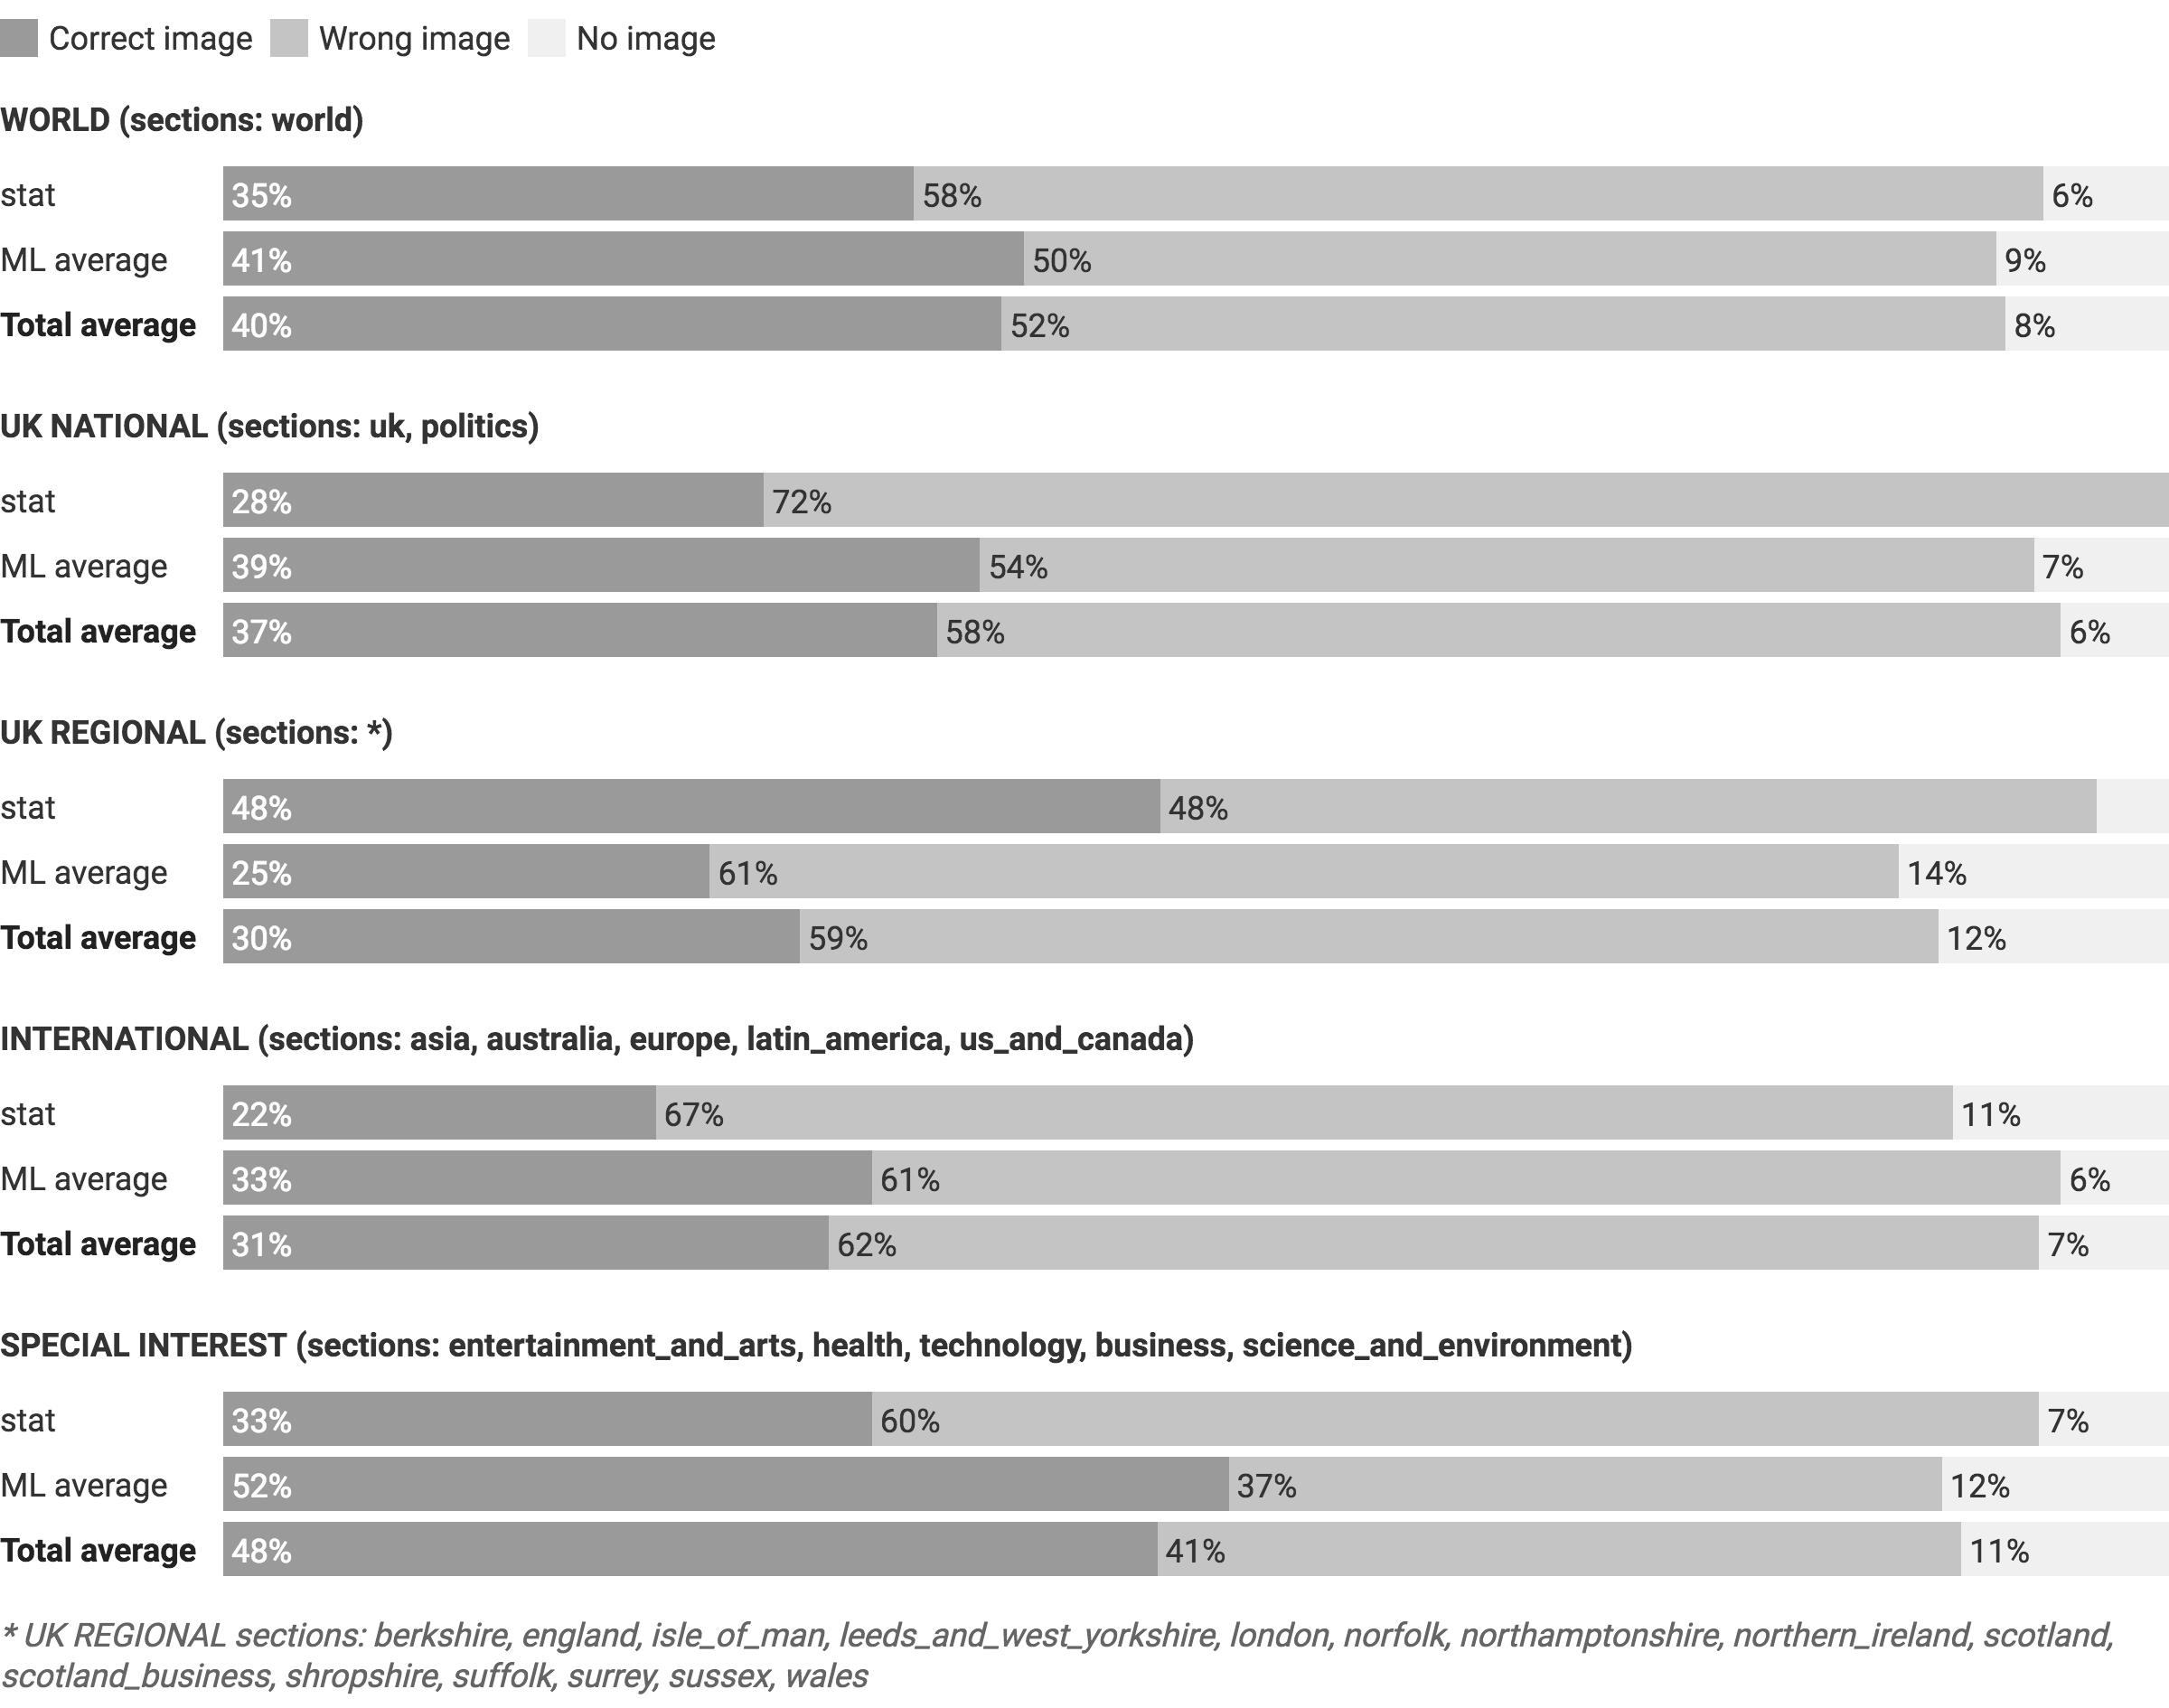
\includegraphics[width=\columnwidth]{fig-perf-per-topic.png}
    \label{fig:perf-per-topic}
\end{figure}

\clearpage

Each of the machine learning approaches in the experiment represents a different combination of term features. This enables a direct comparison of approaches that use a certain feature to approaches that do not, indicating how powerful certain features are. Figure \ref{fig:feature-influence} shows the influence adding certain features had on the performance of the neural networks. 

The most important finding here is the striking effect of the first occurrence feature: Adding it to the networks improved the results by almost 10 percentage points, from 30 \% correct images in the \emph{tf+calais} network to an average of 39,66 \% in all other networks that use first occurrence. This gives evidence to the assumption underlying this feature, namely that the position at which terms occur for the first time in a news article does say a lot about how well it is fit to describe the article's central topic.

The other features do not have an effect as significant as first occurrence. Term frequency on its own seems to have almost no effect at all: Approaches with term frequency performed almost exactly as well as the approach without term frequency. However, term frequency seems to form a powerful pair with first occurrence. Networks that used both features performed better on average (41 \% correct images) than the best network that does not use the two combined (which is \emph{fo+calais} with 37 \% correct images, see Figure \ref{fig:results-overview}).

At first impression, the entity category feature seems to worsen the overall performance of the networks, with only 36.3 \% correct images returned by networks that use it compared to 40 \% in the one that does not. However, it has to be noted that among the networks that use the entity category feature is the negative outlier \emph{tf+calais}. Since the effect of the missing first occurrence feature is overall stronger than the difference for entity category (9.66 percentage points compared to 3.7), it seems likely that this result is biased by the bad performance of \emph{tf+calais}. In fact, adding entity category to the already successful combination \emph{tf+fo} improved it even further, from a rate of 40 \% correct images to 42 \% (see Figure \ref{fig:results-overview}).

\bigskip

Splitting the set of articles into several groups of topically related articles revealed some other interesting patterns. For this purpose, articles were grouped according to the sections they appeared in on BBC News. The resulting topic groups are:

\begin{itemize}
    \setlength\itemsep{0em}
    \item WORLD (containing articles from the "world" section)
    \item UK NATIONAL (containing articles from "uk" and one article from "politics" that was in fact about UK politics)
    \item UK REGIONAL (containing 13 sections representing different regions within the UK)
    \item INTERNATIONAL (containing all sections that represent regions outside the UK, namely "asia", "australia", "europe", "latin\_america" and "us\_and\_canada")
    \item SPECIAL INTEREST (containing topic specific sections such as "health" and "technology")
\end{itemize}

A statistical analysis of the individual groups (shown in Figure \ref{fig:perf-per-topic}) revealed, that the system performed best on SPECIAL INTEREST (48 \% correct images) and WORLD (40 \%) topics on average. It showed its worst average performance in the UK REGIONAL group (30 \%), closely followed by INTERNATIONAL (31 \%). One possible explanation for this is that the majority of images Getty offers come from the anglophone world, especially from the US. Getty is an American image agency that might not cover rural Britain and other parts of the world to the same extent as it covers the US. Queries must therefore be very precise when searching for images from these areas, a task at which the system might have failed a number of times.

However, there are big differences between \emph{stat} and the machine learning approaches. Whereas the neural networks performed slightly better than the statistical approach in almost every topic group, \emph{stat} outperforms the average machine learning approach by far in articles from UK REGIONAL. When it came to British local news, the statistical approach selected almost twice as many factually correct images than the machine learning approach. In fact, this is the highest rate any approach reached on any topic.

One possible explanation for this rather surprising observation is that Open Calais could not make sense of the entities occurring in local news from the UK, which could have blurred the data available for classifying the terms with neural networks. As far as it is known, Open Calais has been "trained by hundreds of Thomson Reuters' Editorial teams" \cite{ThomsonReutersAboutCalais}, i. e. the data used for training Open Calais were articles from the Thomson Reuters news collection. Most of these cover topics of world wide relevance, which means that Open Calais might not have been able to detect entities in local news correctly due to missing training data. However, this does not explain the extraordinarily high percentage of correct articles reached by the statistical approach. The reasons for this remain to be examined.

\bigskip

Another interesting observation arising from the analysis of different topic groups is how the entity category feature influenced the performance \emph{per topic}. As stated above, the networks performed worse in absolute numbers when entity category was added. This applies to all individual topic groups similarly, except for one: In articles from SPECIAL INTEREST, adding entity category actually improved the performance, even when counting the negative outlier \emph{tf+calais}. With entity category, the networks selected 55.5 \% factually correct images on average, without it only 40 \% of images were correct. This might be due to the fact that Open Calais is specialised on industry-related topics with entities such as companies, products and industry terms. These occur particularly often in articles from sections like "business", "technology" and "science and environment" that are all part of this group, leading to a more precise entity recognition.

%______________________________________________________________________

\cleardoublepage

\section{Limitations} \label{Limits}

Before turning to an interpretation of the results presented above as well as some remarks on possible next steps in Section \ref{Conclusion}, the limitations this work has faced will be summed up in the following section. These limitations affected the system design as such as well as the evaluation of its performance. Section \ref{LimitsSystem} will outline the main restrictions the presented system underlies, Section \ref{LimitsEval} will point to the constraints that were imposed on the evaluation.

\subsection{System Limitations} \label{LimitsSystem}

One of the big challenges in implementing the system was generating a set of data precise enough for neural networks to learn from it how to detect meaningful search terms among a huge number of meaningless terms. Defining each term that occurs somewhere in the image description as an image keyword was a workaround that performed surprisingly well - considering that image descriptions often contain several words that are not directly related to the image content, such as the photographer's name or other meta data. However, it can be assumed that there is a significant amount of noise in the data. Using properly labelled images or actual search queries - both of which are not available at the time of writing - could have improved the training data significantly.

Another related issue that might have affected the classification performance is the restricted number of term features. Having to drop part-of-speech and paragraph type as features left the final proposal with only two features per term in the statistical approach and three features maximum in the machine learning approach. This is not to say that additional features would have improved the system's performance \emph{per se}, yet there is room for exploring the effects of features such as term length, the position of a term within a sentence or features describing relations to other terms. Not only time constraints prohibited the introduction of further features, but also computational limitations: A growing number of features would have increased computational complexity for training the networks significantly.

One part of the system that could not be regulated at all is the Getty image search. Since Getty does not expose the algorithms responsible for querying their database, there was no information available as to how well certain search queries were suited for this specific database. Using Getty as an image database black box was a deliberate design decision intended to reduce implementation complexity and keep the proposal as use-case agnostic as possible. However, information about how queries are processed internally could have enabled more detailed improvements, especially regarding the query generation step of the image selection process.

In its current state, the system always selects the first image the API returns. This is dangerous and potentially limits performance, since it leaves much of the decision to Getty's sorting algorithm and - to some extent - coincidence. Furthermore, human editors always rely on their subjective comparison of different images and select the one they think fits the article best. It can be assumed that emulating these decision processes could significantly increase the chance that correct - and maybe even visually attractive - images are selected. As seen in Section \ref{EvalFacts}, editors employ a rather fixed set of criteria during this process. Extending the system to consider these criteria, however, would mean a fundamental change to this proposal, with each criterion leaving lots of room for research on its own.

Another limitation affects the semantic content of the processed articles. The system in its current state only considers those terms that occur in the article literally. It is though possible that in some cases considering synonyms would have been beneficial to the system: Sometimes a synonym might have been the better search term. And sometimes synonyms could have helped to better match article terms and image description, since it is not guaranteed that BBC and Getty use the same terminology in every case.

\subsection{Research Design Limitations} \label{LimitsEval}

The evaluation method applied in this work was designed to be quickly applicable for a big number of articles and approaches. It can be regarded as a first indication as to how well the approaches performed, but never should it be interpreted as a comprehensive measure for the quality of an image selection system. The major limitations are outlined below.

As stated above, professionals apply a wide range of selection criteria to news images. The evaluation at hand examines the most important of them, namely factual correctness, yet still leaves out the majority of criteria that decide on the quality of an image. In order to gain better insight in how well the system performs compared to human editors, it seems feasible to extend the evaluation to other concepts such as visual attractiveness of an image, its compatibility with the headline or matching of moods between article and image. Since these concepts are neither easily definable nor quantifiable in an objective way, recruiting professional journalists as assessors would be vital for such an evaluation to succeed.

What is more, it is not just image curation that plays a role in quality assessment, but also how these images are perceived. As argued in Section \ref{TheoryPerception}, images have great influence on the way readers perceive the news and the mental models they derive from them. None of this is taken account for by measuring only factual correctness of image selections. Experiments and surveys among news readers could help answering central questions arising from automating image selection: How does the proposed system change the way the news are read and perceived? How well do the selected images catch reader's attention, and how well do they improve their recall of the news? All of this are central aspects of quality that can be assessed in future research.

One last limiting factor is the number of examined articles. For this work, 100 articles were evaluated with five different approaches, resulting in 500 individual classifications. This sample size is reasonable for detecting global effects. But when it comes to splitting the sample into different topic groups, a bigger sample could have increased precision especially in small topic groups (e. g. INTERNATIONAL consisted of merely 9 articles in the evaluation on hand).

%______________________________________________________________________

\cleardoublepage

\section{Conclusion} \label{Conclusion}

This work has proposed a system that automatically selects images for news articles by applying simple keyword extraction mechanisms to an article to generate a search query for an image database. The system was designed to be applicable in practice and uses a real-world image database as well as a sample of real-world articles, while still remaining general enough to plug in different keyword extraction methods as well as different data sources for articles and images.

Before the actual system was presented, a review of literature and prior research has revealed important aspects of news and image perception as well as the most influential works that led up to the design of the system. It was found that images play an important role in how news are interpreted by the readers and that their addition supports reader's recall of a story. It was therefore argued that automating this task can not only increase newsroom productivity but also help news publishers make their content more memorable and attractive. Subsequently, a summary of three influential approaches was given, highlighting aspects that inspired the design of this proposal.

In the following comprehensive design report, the system and all related components were outlined and all major design decisions were motivated on the basis of observations made during development. The core part of the system is an image selection pipeline that ranks the terms of an article and generates an image query from the highest ranked terms. It ranks the terms according to three characteristics: term frequency, first occurrence and entity category. Two different ranking approaches were introduced: A computationally efficient statistical approach that calculates predictions with a simple formula, and a more complex machine learning approach based on feedforward neural networks. The networks are pre-trained using a matching of article terms and image descriptions as training data.

In a final evaluation, an attempt was made to compare different approaches systematically according to the rate of factually correct images they select. Five approaches were compared: the statistical approach and four variations of the machine learning approach that use different combinations of the three term characteristics to rank terms. It was found that the neural networks performed slightly better than the statistical calculation on average. The best performing approach was the network that uses all three term features. First occurrence was identified to be very beneficial for the outcome of the system. Term frequency and entity category had less positive impact, yet overall they contributed to improving the system's performance. When comparing different article topics, the observation was made that the statistical approach drastically outperformed the machine learning approaches on local news, but was inferior in all other topic groups.

\bigskip

The most important upshot of this work is that the system in its present form needs more refinement to actually be used in production. With a peak performance of 42 \% factually correct images, not even counting aesthetic aspects or environmental factors such as the intended orientation, it would probably not increase productivity to a particularly high extent. However, several interesting conclusions can be drawn from the experiences made.

The choice of features has proved to be valid according to the evaluation results. Combining all three has resulted in the highest factual accuracy, which indicates that they represent the right knowledge required for ranking the terms. It remains unclear, however, whether it is necessary to invest computational power in the training of neural networks or if similar results could be achieved with a statistical calculation. A direct comparison of both approaches was not possible in this work because one feature, entity category, could only be used in the machine learning approach by definition. The average results indicate though that performance does not increase significantly when neural networks are used.

Regarding individual term features, the most striking finding is the great impact of the first occurrence feature. One central outcome of this work is that the position at which a term is first mentioned in a news article plays a big role in how well it is suited as an image search term. As mentioned above, this is most likely due to the "inverted pyramid" style that puts the central information at the beginning of an article and still seems to influence present day news writing.

Term frequency does, of course, correlate: The earlier a term is mentioned, the higher the chances are that it is mentioned again. Surprisingly though, term frequency on its own seems to have almost no effect at all. It is only in conjunction with first occurrence that term frequency shows positive impact on the factual correctness of image selections.

The conclusion for entity categories as feature is mixed: On the one hand it can be argued that entity categories actually improved the \emph{tf+fo} network, making \emph{tf+fo+calais} the most successful network. On the other hand, this improvement was slight and the average performance did even decrease when adding entity categories. It remains to be examined whether significant improvements can actually be achieved with this kind of classification.

Other interesting conclusions have arisen from the thematic analysis of the results: The proposed system performed best on articles from the "world" section and several special interest sections. Even though this may be caused by Getty's varying amount of coverage for different topics, this suggests that news with a regional focus are not an easy field for the system and that in its current state it is best applied in region-independent news. This does however not explain why the statistical approach performed exceedingly well just on local British news, a phenomenon that requires more detailed investigation in future research.

\bigskip

These conclusions point in various directions for further refinement of the system. Based on the finding in the thematic analysis, a classification of articles according to topics seems reasonable. This would enable the system to treat different topic groups in a different way - for example by using only statistical methods on local news. Open Calais could in fact be a valuable resource for this purpose: Besides the entity recognition, the service returns so called "Social Tags" that "attempt to emulate how a person would tag a specific piece of content" \cite[p. 11]{ThomsonReuters2018ThomsonGuide}. These tags could be used to determine the type of article the system deals with.

As stated in Section \ref{LimitsSystem}, choosing one image from a list of query results instead of always choosing the first image could help emulate human selection behaviour in a more natural way. For this purpose, an image ranking method could be implemented that rates the images before selecting the highest rated. Inspiration could be drawn from the approaches by Joshi et al. \cite{Joshi2006TheIllustration} and Delgado et al. \cite{Delgado2010AutomatedExperience} that were introduced in Section \ref{TheoryTech} and both implement an image ranking.

Section \ref{LimitsSystem} revealed that the training data used in this system might not have been precise enough for the neural networks to fully grasp what makes a good search term. One obvious way to tackle this is to collect actual search terms human editors use in image databases. This would be both time consuming and hard to implement, since it would require an integration into editor's everyday workflows or an extensive laboratory experiment. Another approach might be more feasible: Switching from feedforward neural networks to recurrent neural networks would introduce the possibility of feedback loops. The networks could then iteratively learn from feedback humans give them on their selections, for example from editors using the systems in their regular work. In doing so, they would help the networks approximate the human intuition of a good search term, hopefully leading to higher precision.

Future research should furthermore examine new ways of characterising a term: Does the length of a term play a role when it comes to extracting search queries? Do other position features such as within-sentence position or within-paragraph position have a similarly big effect as first occurrence? How do neighbouring terms affect the suitability of a term as search term? And can search queries be improved by replacing terms with synonyms where applicable?

Further room for improvement exists when it comes to evaluating the system. As stated in Section \ref{LimitsEval}, factual correctness can be regarded as a first indication of the system's performance, but deeper investigations have to follow: How well does the system approximate the criteria professional photo editors apply when selecting images? What are their attitudes towards systems like this? Surveys and experiments with professionals can give hints towards answering these questions. How does the system influence reader's perception of the news? Does it change their perception at all? And is there a visible difference between images selected by humans and images selected by the machine? These and related questions can only be answered by collecting feedback from the affected audience.

Finally, creating these kinds of systems has ethical implications. It has to be debated to which extent news publishers should rely on an autonomous system like this, even if it were flawless in the execution of its task. By design, this system is not aware of the impact its selections might have on the readers. Neither does it know about possibly harmful content, nor about framing effects it could cause. Even though it only tries to imitate human behaviour, it can not be guaranteed that it will always act as wise as a human would. This work therefore strongly discourages the use of systems like this in a completely autonomous fashion. Especially in journalism, where minor mistakes can cause great harm and trust is easily lost, it seems advisable to subject automated image selection to human supervision.

\bigskip

However, this work has shown the potential that lies in automation: Selecting an image takes seconds with the current implementation. Even if it was only used as a suggestion tool for editors, and even with its current success rate, it may be assumed that newsrooms can benefit from it. What is more, there exist various paths for further improving the system. Future research has yet to show to which extend these kinds of systems can actually augment the image selection process. But in times of increasing competition in the media sector, publishers are well advised to invest in new forms of content generation. This work and potential future continuations can be a meaningful contribution to this development.

%\_____________________________________________________________________

\cleardoublepage

\begin{appendix}

\section{Source Code} \label{AppendixCode}

The proposed system has been implemented in JavaScript for Node.js for research reasons. It consists of four open source projects that can either be found on the CD attached to the printed version of this thesis or under the links provided below.

\begin{table}[h]
    \centering
    \begin{tabular}{|c|p{4.5cm}|c|}
        \hline
        \textbf{Project Name} & \textbf{Description} & \textbf{URL} \\
        \hline
        gettygetter & Scraping application for collecting data from BBC News, Getty Images and Open Calais & \url{https://github.com/mgschoen/gettygetter} \\
        \hline
        picpic-core & Collection of tools for preprocessing, keyword extraction and training of neural networks & \url{https://github.com/mgschoen/picpic-core} \\
        \hline
        picpic-api & Public REST interface that applies the image selection pipeline to the corpus collected with gettygetter & \url{https://github.com/mgschoen/picpic-api} \\
        \hline
        picpic-explorer & Statically served web frontend for interacting with picpic-api & \url{https://github.com/mgschoen/picpic-explorer} \\
        \hline
    \end{tabular}
    \label{table:source-code}
\end{table}

\clearpage

\section{List of Stopwords} \label{AppendixStopwords}

\emph{This is the global list of stopwords that was used in the entire application. The character "," in the following list denotes a word separator.}

\bigskip

\noindent about, above, after, again, all, also, am, an, and, another, any, are, as, at, be, because, been, before, being, below, between, both, but, by, came, can, cannot, come, could, did, do, does, doing, during, each, few, for, from, further, get, got, has, had, he, have, her, here, him, himself, his, how, if, in, into, is, it, its, itself, like, make, many, me, might, more, most, much, must, my, myself, never, new, now, of, on, only, or, other, our, ours, ourselves, out, over, own, said, same, see, she, should, since, so, some, still, such, take, than, that, the, their, theirs, them, themselves, then, there, these, they, this, those, through, to, too, under, until, up, very, was, way, we, well, were, what, where, when, which, while, who, whom, with, would, why, you, your, yours, yourself, a, b, c, d, e, f, g, h, i, j, k, l, m, n, o, p, q, r, s, t, u, v, w, x, y, z, \$, 1, 2, 3, 4, 5, 6, 7, 8, 9, 0, \_

\clearpage

\section{Grouping of Open Calais Entity Types} \label{AppendixEntcats}

\begin{table}[h!]
    \centering
    \begin{tabular}{|c|p{10cm}|}
        \hline
        \textbf{Entity Category}& \textbf{Associated Entity Types} \\
        \hline
        Event                   & \nohyphens{Anniversary, Date, EntertainmentAwardEvent, Holiday, PoliticalEvent, SportsEvent, SportsGame, SportsLeague, TVShow} \\
        \hline
        HumanProtagonist        & Editor, Journalist, MusicGroup, Person \\
        \hline
        OrganizationProtagonist & Company, Organization \\
        \hline
        Position                & Position \\
        \hline
        Location                & \nohyphens{City, Continent, Country, Facility, NaturalFeature, ProvinceOrState, Region} \\
        \hline
        Product                 & \nohyphens{Movie, MusicAlbum, OperatingSystem, PharmaceuticalDrug, Product, ProgrammingLanguage, PublishedMedium, RadioProgram, RadioStation, Technology, TVShow, TVStation} \\
        \hline
        Other                   & \nohyphens{EmailAddress, FaxNumber, IndustryTerm, MarketIndex, MedicalCondition, MedicalTreatment, PhoneNumber, URL} \\
        \hline
    \end{tabular}
    \label{table:entity-groups}
\end{table}

\end{appendix}

%\_____________________________________________________________________

\cleardoublepage
\fancyhead[LE,RO,LO,RE]{} % Keine Kopfzeile mehr oben auf jeder Seite
\section*{Contents of the Attached CD}

\emph{The attached CD contains the following folders:}

\begin{itemize}
    \item \lstinline{/code} - the source code of the proposed system
    \item \lstinline{/corpus} - all data collected from BBC News, Getty Images and Open Calais until submission of this work
    \item \lstinline{/evaluation} - an overview of the evaluation results
    \item \lstinline{/literature} - all references that were available online at the time of submission
    \item \lstinline{/thesis} - this thesis in LaTeX and PDF format
\end{itemize}

%______________________________________________________________________

\cleardoublepage
%\begin{thebibliography}{99}

%\bibitem{Ivory01}

%  M.\ Y.\ Ivory, M.\ Hearts:
%  \href{http://www.ischool.washington.edu/myivory/thesis/thesis.pdf}{%
%    An Empirical Foundation for Automated Web Interface Evaluation}.
%  Ph.D. thesis, University of California at Berkeley, 2001


%\cleardoublepage
%\hspace{-\leftmargin}{\Large\bfseries Web-Referenzen} % Wüster Hack %-|

%\bibitem{NielsenAlertbox}

%  J.\ Nielsen: Alertbox: Current Issues in Web Usability
%  \url{http://useit.com/alertbox/}, accessed April~24, 2005.

%\end{thebibliography}

\bibliographystyle{plain}
\bibliography{mendeley}

\end{document}
